%% Use the option review to obtain double line spacing 
%% \documentclass[preprint,review,12pt]{elsarticle} 
%% Use the options 1p,twocolumn; 3p; 3p,twocolumn; 5p; or 5p,twocolumn 
%% for a journal layout: 
%% \documentclass[final,1p,times]{elsarticle} 
%% \documentclass[final,1p,times,twocolumn]{elsarticle} 
%% \documentclass[final,3p,times]{elsarticle} 
%%\documentclass[final,3p,times,twocolumn]{elsarticle} 
%% \documentclass[final,5p,times]{elsarticle} 
 \documentclass[final,5p,times,twocolumn]{elsarticle} 

\usepackage{amsfonts}
\usepackage{amsmath}
\usepackage{amssymb}
\usepackage{booktabs}
\usepackage{caption}
\usepackage{color}
\usepackage{comment}
\usepackage{graphicx}
\usepackage{hyperref}
\usepackage[utf8]{inputenc} % allows using accents directly in text, like ÔøΩ
\usepackage{subfig}
\usepackage{xspace}


\captionsetup{justification=raggedright,
singlelinecheck=false
}

\newcommand{\pygbe}{\texttt{PyGBe}\xspace}
\newcommand{\gb}{{\small G\,B1\,D4$^\prime$}\xspace}
\newcommand{\gmres}{\textsc{gmres}\xspace}
\newcommand{\bem}{\textsc{bem}\xspace}
\newcommand{\ses}{\textsc{ses}\xspace}
\newcommand{\sam}{\textsc{sam}}
\newcommand{\gpu}{\textsc{gpu}}
\newcommand{\cpu}{\textsc{cpu}}
\newcommand{\apbs}{\textsc{apbs}\xspace}
\newcommand{\nvidia}{\textsc{nvidia}\xspace}
\newcommand{\msms}{\texttt{\textsc{msms}}\xspace}
\newcommand{\amber}{\texttt{\textsc{amber}}\xspace}
\newcommand{\ccby}{\textsc{cc-by}\xspace}

\graphicspath{{figs/}} %  PATH to figure files-- change to ./ for submission

%% The lineno packages adds line numbers. Start line numbering with
%% \begin{linenumbers}, end it with \end{linenumbers}. Or switch it on
%% for the whole article with \linenumbers after \end{frontmatter}.
%% \usepackage{lineno}

%% natbib.sty is loaded by default. However, natbib options can be
%% provided with \biboptions{...} command. Following options are
%% valid:

%%   round  -  round parentheses are used (default)
%%   square -  square brackets are used   [option]
%%   curly  -  curly braces are used      {option}
%%   angle  -  angle brackets are used    <option>
%%   semicolon  -  multiple citations separated by semi-colon
%%   colon  - same as semicolon, an earlier confusion
%%   comma  -  separated by comma
%%   numbers-  selects numerical citations
%%   super  -  numerical citations as superscripts
%%   sort   -  sorts multiple citations according to order in ref. list
%%   sort&compress   -  like sort, but also compresses numerical citations
%%   compress - compresses without sorting
%%
%% \biboptions{comma,round}

% \biboptions{}


\journal{Computer Physics Communications}

\begin{document}

\begin{frontmatter}

%% Title, authors and addresses

%% use the tnoteref command within \title for footnotes;
%% use the tnotetext command for the associated footnote;
%% use the fnref command within \author or \address for footnotes;
%% use the fntext command for the associated footnote;
%% use the corref command within \author for corresponding author footnotes;
%% use the cortext command for the associated footnote;
%% use the ead command for the email address,
%% and the form \ead[url] for the home page:
%%
%% \title{Title\tnoteref{label1}}
%% \tnotetext[label1]{}
%% \author{Name\corref{cor1}\fnref{label2}}
%% \ead{email address}
%% \ead[url]{home page}
%% \fntext[label2]{}
%% \cortext[cor1]{}
%% \address{Address\fnref{label3}}
%% \fntext[label3]{}

\title{Poisson-Boltzmann model for protein-surface electrostatic interactions and grid-convergence study using the \pygbe code}

\author[bu,usm]{Christopher D. Cooper\corref{cdc}}
\ead{cdcooper@bu.edu}

\author[gwu]{Lorena A.~Barba\corref{lab}}
\ead{labarba@gwu.edu}

\address[bu]{Department of Mechanical Engineering, Boston University, Boston, MA.}
\address[usm]{Department of Mechanical Engineering, Universidad T\'ecnica Federico Santa Mar\'ia, Valpara\'iso, Chile.}
\address[gwu]{Department of Mechanical \& Aerospace Engineering, The George Washington University, Washington, D.C.}
\cortext[lab]{\href{mailto:labarba@gwu.edu}{labarba@gwu.edu}}

%\date{\today}

\begin{abstract}

Interactions between surfaces and proteins occur in many vital processes and are crucial in biotechnology: the ability to control specific interactions is essential in fields like biomaterials, biomedical implants and biosensors. In the latter case, biosensor sensitivity hinges on ligand proteins adsorbing on bioactive surfaces with a favorable orientation, exposing reaction sites to target molecules.
Protein adsorption, being a free-energy-driven process, is difficult to study experimentally. This paper develops and evaluates a computational model to study electrostatic interactions of proteins and charged nanosurfaces, via the Poisson-Boltzmann equation.
We derived an analytical solution for a spherical charged surface interacting with a spherical molecule, extended the implicit-solvent model used in the open-source code PyGBe to include surfaces of imposed charge, then completed a grid-convergence study to build evidence on the correctness and usefulness of our approach.
PyGBe solves the boundary integral formulation of the Poisson-Boltzmann equation, discretized with surface elements. At its core is a treecode-accelerated Krylov iterative solver, resulting in $O(N \log N)$ scaling, and further acceleration on hardware via multi-threaded execution on \gpu s. It computes solvation, surface and interaction free energies, providing a framework for studying the effect of electrostatics on adsorption.
In the grid-convergence study with the analytical solution, the error decays with the average area of the boundary elements, i.e., the method is $O(1/N)$, which is consistent with our previous verification studies using PyGBe.
We also studied grid-convergence using a real molecular geometry (protein G~B1~D4'), in this case using Richardson extrapolation (in the absence of an analytical solution) and confirm the $O(1/N)$ scaling in this case.
PyGBe is open-source under an MIT license. In addition, to supplement this paper we prepared ``reproducibility packages'' consisting of running and post-processing scripts in Python to allow replication of the grid-convergence studies, all the way to generating the final plots, all with a single command.
\end{abstract}

\begin{keyword}
biomolecular electrostatics \sep protein surface interaction \sep implicit solvent \sep Poisson-Boltzmann \sep boundary element method \sep treecode \sep Python \sep CUDA

%% MSC codes here, in the form: \MSC code \sep code
%% or \MSC[2008] code \sep code (2000 is the default)

\end{keyword}

\end{frontmatter}

% Body of paper.

\section{Introduction}\label{sec:intro}
%!TEX root = CooperBarba2014.tex

Interactions between proteins and solid surfaces are ubiquitous in many biological processes. Adsorption plays a role in natural activity, like blood coagulation, and is also a key mechanism in biotechnologies like tissue engineering, biomedical implants and biosensors.
A full understanding of protein-surface interactions has remained elusive \cite{Gray2004,RabeVerdesSeegel2011}, but adsorption mechanisms are governed by surface energy and often the dominant effect is electrostatics.

Protein electrostatics can be studied via modeling approaches using the Poisson-Boltzmann equation and implicit-solvent representations. These models  are popular for computing solvation energies in protein systems \cite{RouxSimonson1999,Bardhan2012}, but few studies have included the effect of surfaces. Lenhoff and co-workers studied surface-protein interactions using continuum models discretized with boundary-element \cite{YoonLenhoff1992,RothLenhoff1993,AsthagiriLenhoff1997} and finite-difference methods \cite{YaoLenhoff2004,YaoLenhoff2005}, in the context of ion-exchange chromatography. They realized that van der Waals effects can be neglected for realistic molecular geometries \cite{RothNealLenhoff1996} and that the model is adequate as long as conformational changes in the protein are slight \cite{YaoLenhoff2004,YaoLenhoff2005}. 

The aim of this work is to develop and assess a computational model to simulate proteins near engineered surfaces of fixed charge, using implicit-solvent electrostatics.
We have added the capability of modeling a protein near a charged surface to our code \pygbe, an open-source code\footnote{\url{https://github.com/barbagroup/pygbe}}  that solves the Poisson-Boltzmann equations via an integral formulation, using a fast multipole algorithm and \gpu\ hardware acceleration.  Previously, we verified and validated \pygbe in its use to obtain solvation and binding energies, by comparing with analytical solutions of the equations and with results obtained using the well-known \apbs software \cite{CooperBarba-share154331,CooperBardhanBarba2013}. 
In the present work, we derived an analytical solution for a spherical molecule interacting with a spherical surface of prescribed charge, and used it to verify the code in its new application and study numerical convergence.
Using the newly extended code, we also studied the interaction between protein GB1 D4' and a solid surface of imposed charge, with the goal of comparing our results with published studies using both experimental methods\cite{BaioWeidnerBaughGambleStaytonCastner2012} and molecular simulations.\cite{LiuLiaoZhou2013}

We anticipate our new modeling tool to be useful for studying the behavior of proteins as they adsorb on surfaces that have been functionalized with  self-assembled monolayers (\sam), for example, which are modeled as a surface with prescribed charge within an implicit-solvent framework. 
One application is biosensing, where the target molecule is attached to the sensor through a ligand molecule (in many cases an antibody). The performance of the biosensor is then crucially affected by the orientation of the ligand molecule \cite{TajimaTakaiIshihara2011,TrillingBeekwilderZuilhof2013}, whose binding sites must be physically accessible to the target molecule. Studies of protein orientation near charged surfaces using this model could thus aid the design of better biosensors. We explore this application in a companion publication that studies orientation of an antibody near a surface and the effect of changing the conditions of surface preparation (charge and ionic strength).\cite{CooperBarba2015b}. Here, we present the details of the new analytical solution for charged surface and molecule of spherical geometry, grid-convergence studies for the interaction free energy in this case, and grid-convergence studies for protein GB1 alone and interacting with a charged surface. The detailed analysis of the model is complemented with a diligent effort for reproducibility and we deposit both input and results data in accessible and permanent archival storage.


\section{Implicit-solvent model for proteins near charged surfaces} \label{sec:implicit_solvent}
    %!TEX root = CooperBarba2014.tex

The implicit-solvent model describes a molecular system as a set of continuum dielectric regions, and computes the mean-field potential using electrostatics. 
For the case where a protein is dissolved in a solvent, we require two of such regions: inside and outside the protein, interfaced by the solvent-excluded surface (\ses). 
The \ses determines the closest a water molecule can get to the protein, and we generate it by rolling a spherical probe of the size of a water molecule around the protein. 
The dielectric constant inside the protein is low ($\epsilon= 2\text{ to }4$) and there are point charges to mimic the charge distribution, placed at the atoms' locations. On the other hand, the solvent region has the dielectric constant of water $\epsilon \approx 80$, and we need to account for the presence of salt. 
This model results in a system of partial differential equations where the Poisson equation describes the electrostatic potential inside the protein, and the linearized Poisson-Boltzmann equation applies outside the protein. On the \ses, appropriate interface conditions ensure the continuity of the potential and electric displacement.

In this work, we use an extension of the implicit-solvent model to consider the effect of charged surfaces. Such is the case of the setup sketched by Figure \ref{fig:molecule_surface}, which is described mathematically by the following equations:


\begin{align} \label{eq:pde}
\nabla^2 \phi_1(\mathbf{r}) &= - \sum_k \frac{q_k}{\epsilon_1} \delta(\mathbf{r},\mathbf{r}_k) \ \text{ in solute $(\Omega_1)$,}  \nonumber \\ 
\nabla^2\phi_2 (\mathbf{r}) &= \kappa^2 \phi_2(\mathbf{r}) \quad \qquad \ \ \ \text{ in solvent $(\Omega_2)$,}  \nonumber \\ 
\phi_1 &=\phi_2 \nonumber \\ 
\epsilon_1 \frac{\partial \phi_1}{\partial \mathbf{n}} &= \epsilon_2 \frac{\partial \phi_2}{\partial \mathbf{n}}  \ \qquad \qquad \text{ on interface $\Gamma_1$, and} \nonumber \\
-\epsilon_2 \frac{\partial \phi_2}{\partial \mathbf{n}} &= \sigma_0 \qquad \qquad \qquad \text{ on surface $\Gamma_2$} 
\end{align}

\noindent where $\phi_i$ is the electrostatic potential in region $\Omega_i$, which has a permittivity $\epsilon_i$, and $\sigma_0$ is a prescribed charge on the surface. The surface $\Gamma_2$ could correspond to a device such as a biosensor.

\begin{figure}
   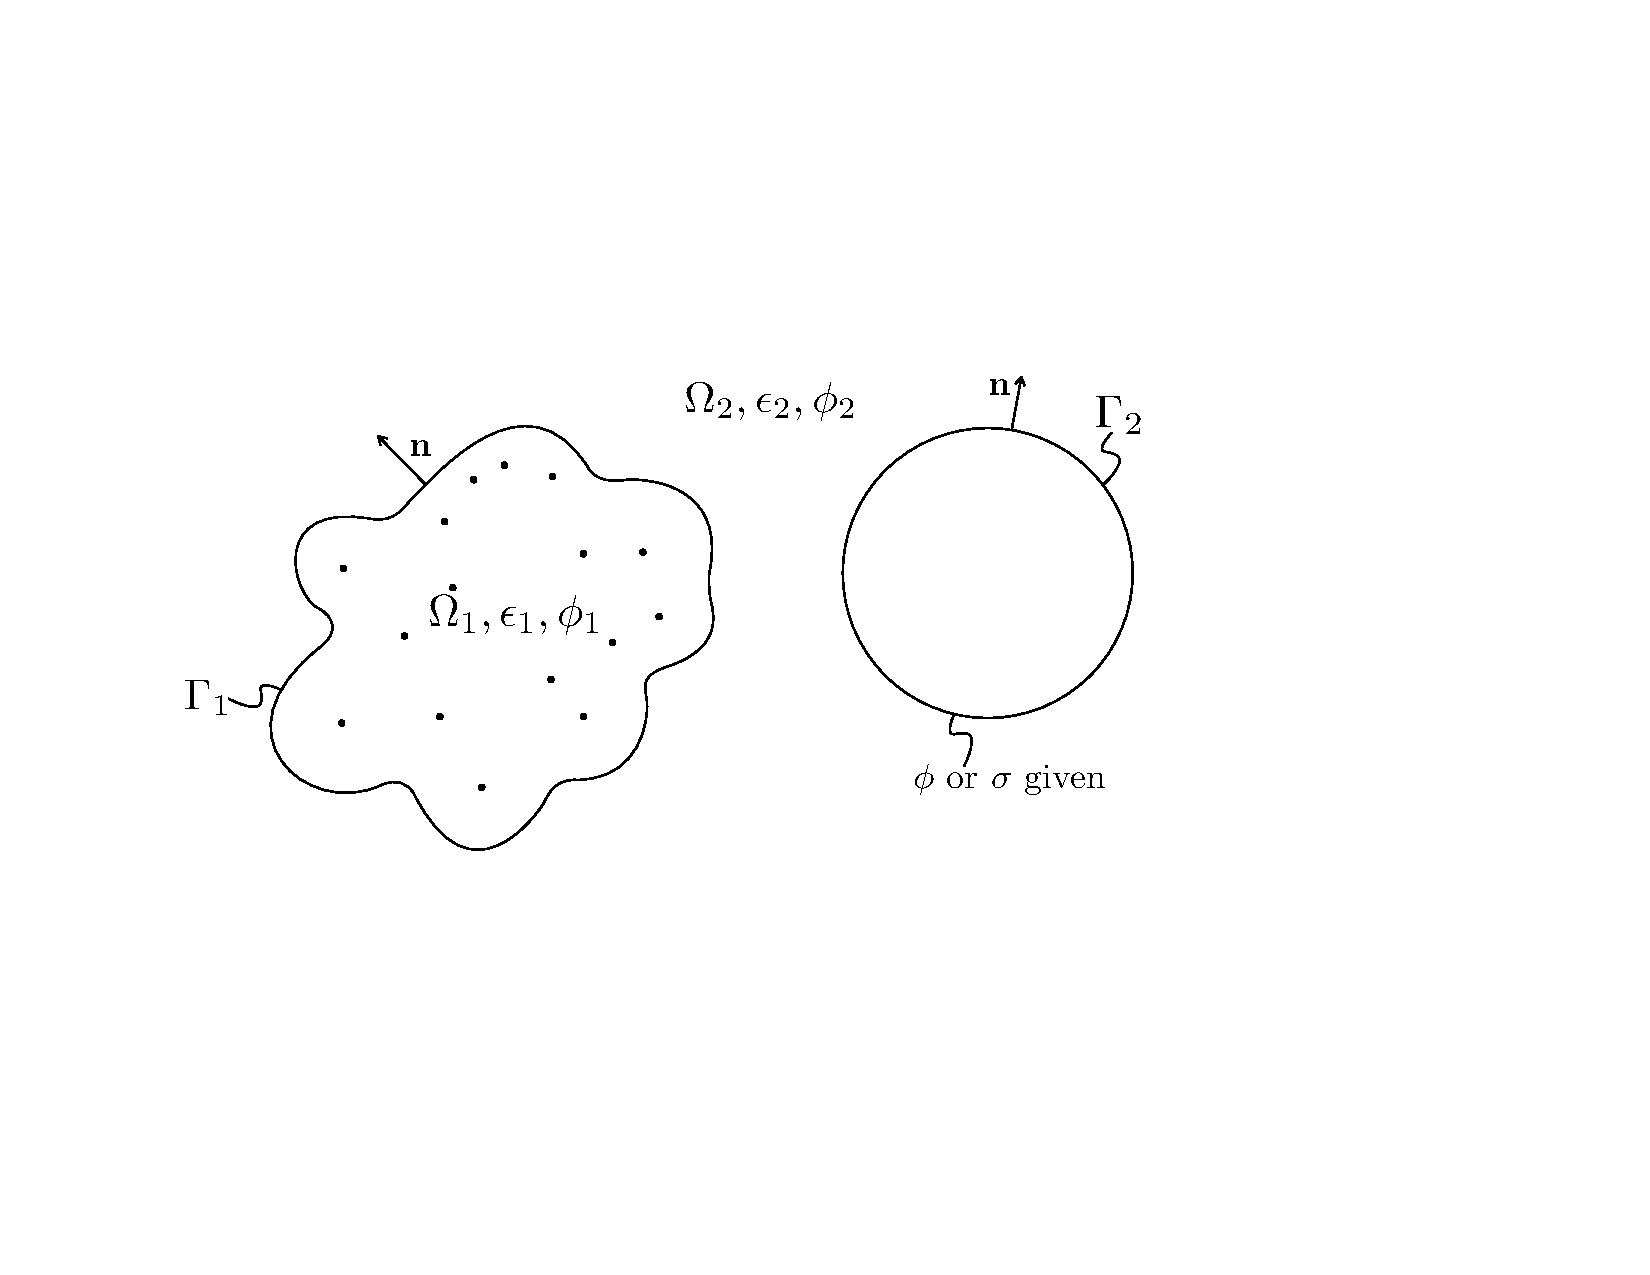
\includegraphics[width=0.45\textwidth]{Figure2.pdf} 
   \caption{Sketch of a molecule interacting with a surface: $\Omega_1$ is the protein, $\Omega_2$ the solvent region, $\Gamma_1$ is the  \ses and $\Gamma_2$ a surface with imposed charge.}
   \label{fig:molecule_surface}
\end{figure}


\paragraph*{Boundary integral formulation} \label{sec:bie}
%!TEX root = CooperBarba-orientation.tex


We apply Green's second identity to the system of partial-differential equations in \eqref{eq:pde}, and evaluate the resulting equations on $\Gamma_1$ and $\Gamma_2$ to obtain the following system of integral equations:
%
\begin{widetext}
\begin{align} \label{eq:integral_eq}
\frac{\phi_{1,\Gamma_1}}{2}+ K_{L}^{\Gamma_1}(\phi_{1,\Gamma_1}) -  V_{L}^{\Gamma_1} \left(\frac{\partial}{\partial \mathbf{n}}\phi_{1,\Gamma_1} \right)  =  
\frac{1}{\epsilon_1} \sum_{k=0}^{N_q} \frac{q_k}{4\pi|\mathbf{r}_{\Gamma_1} - \mathbf{r}_k|} &  \quad \text{on $\Gamma_1$,} \nonumber \\ 
\frac{\phi_{1,\Gamma_1}}{2} - K_{Y}^{\Gamma_1}(\phi_{1,\Gamma_1}) +  \frac{\epsilon_1}{\epsilon_2} V_{Y}^{\Gamma_1} \left( \frac{\partial}{\partial \mathbf{n}} \phi_{1,\Gamma_1} \right) -  
K_{Y}^{\Gamma_1}(\phi_{2,\Gamma_2})  + V_{Y}^{\Gamma_1} \left( -\frac{\sigma_0}{\epsilon_2} \right)  = 0& \quad \text{on $\Gamma_1$,} \nonumber \\ 
- K_{Y}^{\Gamma_2}(\phi_{1,\Gamma_1}) + \frac{\epsilon_1}{\epsilon_2} V_{Y}^{\Gamma_2}  \left( \frac{\partial}{\partial \mathbf{n}} \phi_{1,\Gamma_1} \right) + \frac{\phi_{2,\Gamma_2}}{2} - 
K_{Y}^{\Gamma_2}(\phi_{2,\Gamma_2}) +  V_{Y}^{\Gamma_2} \left( -\frac{\sigma_0}{\epsilon_2} \right)  = 0& \quad \text{on $\Gamma_2$.}
\end{align}
\end{widetext}


\noindent The function $\phi_{i,\Gamma_j} = \phi_i(\mathbf{r}_{\Gamma_j})$ is the electrostatic potential at a point that approaches the surface $\Gamma_j$ from the region $\Omega_i$, and
$K$ and $V$ are known as the single- and double-layer potentials, correspondingly:
%
\begin{align} \label{eq:layers}
K_{L/Y}^{\Gamma_k}(\phi_{i,\Gamma_j}) &= \oint_{\Gamma_j} \frac{\partial}{\partial \mathbf{n}} \left[ G_{L/Y}(\mathbf{r}_{\Gamma_k},\mathbf{r}_{\Gamma_j}) \right]\phi_{i,\Gamma_j} \, \mathrm{d} \Gamma, \nonumber \\
V_{L/Y}^{\Gamma_k} \left( \frac{\partial}{\partial \mathbf{n}} \phi_{i,\Gamma_j} \right) &= \oint_{\Gamma_j} \frac{\partial}{\partial \mathbf{n}} \phi_{i,\Gamma_j} G_{L/Y}(\mathbf{r}_{\Gamma_k},\mathbf{r}_{\Gamma_j})  \, \mathrm{d} \Gamma.
\end{align}

\noindent In Equation \eqref{eq:layers}, $G_L$ and $G_Y$ are the free-space Green's functions of the Poisson and linearized Poisson-Boltzmann equations, respectively. 
The single-layer potential of a distribution $\psi$ on a surface $\Gamma$ evaluated at $\mathbf{r}$, $V^\mathbf{r}(\psi_\Gamma)$, can be interpreted as the potential on $\mathbf{r}$ due to a charge distribution $\psi$ on $\Gamma$. 
Similarly, $K^\mathbf{r}(\psi_\Gamma)$ can be seen as the potential induced by a double layer of charges ($\psi$) with opposite sign at $\Gamma$.

Rearranging terms, we write Equation \eqref{eq:integral_eq} in matrix form, as follows:
%
 \begin{align} \label{eq:matrix_dphi}
 \left[
    \begin{matrix} % or pmatrix or bmatrix or Bmatrix or ...
       \frac{1}{2} + K_{L}^{\Gamma_1} & -V_{L}^{\Gamma_1} & 0 \vspace{0.2cm}\\
       \frac{1}{2} - K_{Y}^{\Gamma_1} &  \frac{\epsilon_1}{\epsilon_2} V_{Y}^{\Gamma_1} & -K_{Y}^{\Gamma_1} \vspace{0.2cm} \\
       - K_{Y}^{\Gamma_2} & \frac{\epsilon_1}{\epsilon_2} V_{Y}^{\Gamma_2} & \left(\frac{1}{2} - K_{Y}^{\Gamma_2}\right) \\
    \end{matrix}
    \right] \left[ 
    \begin{matrix} % or pmatrix or bmatrix or Bmatrix or ...
       \phi_{1,\Gamma_1} \vspace{0.2cm} \\
       \frac{\partial}{\partial \mathbf{n}} \phi_{1,\Gamma_1} \vspace{0.2cm}\\
       \phi_{2,\Gamma_2}\\
    \end{matrix} 
     \right] =   \nonumber \\
    \left[
    \begin{matrix} % or pmatrix or bmatrix or Bmatrix or ...
       \sum_{k=0}^{N_q} \frac{q_k}{4\pi|\mathbf{r}_{\Gamma_1} - \mathbf{r}_k|} \vspace{0.2cm} \\
        V_{Y}^{\Gamma_1} \left( \frac{\sigma_0}{\epsilon_2} \right) \vspace{0.2cm} \\
        V_{Y}^{\Gamma_2} \left( \frac{\sigma_0}{\epsilon_2} \right)
    \end{matrix}
    \right].
 \end{align}

The boundary-integral formulation is not limited to represent the protein with a single surface, but can account for solvent-filled cavities inside the protein region and Stern layers.\cite{CooperBardhanBarba2013} In those cases, more than one surface is required to appropriately represent the protein. 
This implementation follows the guidelines from Altman and co-workers to deal with multiple surfaces.

The boundary-integral formulation of the implicit-solvent model is a popular alternative to compute solvation energies of proteins,\cite{YoonLenhoff1990, Juffer1991a, LuETal2006, BajajETal2011, AltmanBardhanWhiteTidor09, GengKrasny2013, CooperBardhanBarba2013} but the effect of charged surfaces has rarely been considered. The only work that we know of that does include these effects is limited to plane, infinite surfaces.\cite{YoonLenhoff1992} 



%=============
\section{Methods}\label{sec:methods}

%!TEX root = CooperBarba2014.tex

\subsection{Discretization}

To numerically solve the system in \eqref{eq:matrix_dphi}, we discretize the boundaries into flat triangular panels and assume that $\phi$ and $\frac{\partial \phi}{\partial \mathbf{n}}$ are constant within those panels. The discretized form of the integral operators is as follows:
%
\begin{align} \label{eq:layers_disc}
&K_{L,\text{disc}}^{\mathbf{r}_i}\left(\phi(\mathbf{r}_{\Gamma})\right) =  \sum_{j=1}^{N_p}\phi(\mathbf{r}_{\Gamma_j})\int_{\Gamma_j} \frac{\partial}{\partial \mathbf{n}} \left[ G_L(\mathbf{r}_{i},\mathbf{r}_{\Gamma_j}) \right]\mathrm{d} \Gamma_j,  \nonumber \\
&V_{L,\text{disc}}^{\mathbf{r}_i} \left( \frac{\partial}{\partial \mathbf{n}} \phi(\mathbf{r}_{\Gamma}) \right) = \sum_{j=1}^{N_p} \frac{\partial}{\partial \mathbf{n}} \phi(\mathbf{r}_{\Gamma_j}) \int_{\Gamma_j} G_L(\mathbf{r}_{i},\mathbf{r}_{\Gamma_j})  \mathrm{d} \Gamma_j,
\end{align}

\noindent where $N_p$ is the number of discretization elements on $\Gamma$, and $\phi(\mathbf{r}_{\Gamma_j})$ and $\frac{\partial}{\partial \mathbf{n}} \phi(\mathbf{r}_{\Gamma_j})$ are the constant values of $\phi$ and $\frac{\partial \phi}{\partial \mathbf{n}}$ on panel $\Gamma_j$ (we are somewhat abusing the nomenclature here by reusing the symbol $\Gamma$, which previously referred to the complete surface). By collocating $\mathbf{r}_i$ on the center of each panel, we get a linear system of equations that look just like \eqref{eq:matrix_phi} or \eqref{eq:matrix_dphi}, but the coefficient matrix is formed by sub-matrices of size $N_p \times N_p$ rather than integral operators. Each element of a sub-matrix is an integral over one panel $\Gamma_j$, with $\mathbf{r}_i$ located at the center of the collocation panel $\Gamma_i$, as follows:

\begin{align} \label{eq:layers_element}
K_{L,ij} &= \int_{\Gamma_j} \frac{\partial}{\partial \mathbf{n}} \left[ G_L(\mathbf{r}_{\Gamma_i},\mathbf{r}_{\Gamma_j}) \right]\mathrm{d} \Gamma_j, \nonumber \\
V_{L,ij} &= \int_{\Gamma_j} G_L(\mathbf{r}_{\Gamma_i},\mathbf{r}_{\Gamma_j})  \mathrm{d} \Gamma_j.
\end{align}

The terms on the right-hand side and the unknown vectors in the discretized form of Equation \eqref{eq:matrix_phi} are sub-vectors of size $N_p$. In this case, each element is the evaluation on the collocation panel $\Gamma_i$, written as
%
\begin{align} \label{eq:vector_disc}
\phi_{1,\Gamma_1} &= \phi_1(\mathbf{r}_i), \nonumber \\
\frac{\partial}{\partial \mathbf{n}}\phi_{1,\Gamma_1} &= \frac{\partial}{\partial \mathbf{n}}\phi_1(\mathbf{r}_i), \nonumber \\
\sum_{k=0}^{N_q} \frac{q}{4\pi|\mathbf{r}_{\Gamma_1} - \mathbf{r}_k|} &= \sum_{k=0}^{N_q} \frac{q}{4\pi|\mathbf{r}_i - \mathbf{r}_k|},
\end{align}

\noindent where $\mathbf{r}_i$ is located at the center of panel $\Gamma_i$.

In our numerical solution, integrals are calculated in three possible ways, depending on how close the panel is to the collocation point. When the collocation point is inside the element being integrated, we use a semi-analytical technique \cite[p.~49, ff.]{HessSmith1967}, with Gauss points placed along the edges of the element. If the integrated element is closer than $2L$ from the collocation point ---where $L = \sqrt{2\cdot \text{Area}}$--- we use a fine Gauss quadrature rule, with 19 or more points per element. Beyond a distance of $2L$, elements have only 1, 3, 4 or 7 Gauss points, depending on the case.

\subsection{Treecode-accelerated boundary element method}

Most modern implementations of the boundary element method (\bem) use Krylov methods to solve the linear system, usually a general minimal residual method (\gmres), which is agnostic to the structure of the matrix. In practice, Krylov solvers for \bem require $O(n \cdot N_p^2)$ operations to obtain the unknown vector, where $n$ is the number of iterations to get a desired residual, and is much smaller than $N_p$. The $O(N^2)$ scaling is given by a matrix-vector product (with a dense matrix) done in every iteration; this is the most time-consuming part of the algorithm, and makes \bem prohibitive for more than a few thousand discretization elements. 

But when we inspect the approximation of the integrals in  \eqref{eq:layers_element} with Gauss quadrature rules, we see that the matrix-vector product has the form of an $N$-body problem, similar to gravitational potential calculations in planetary systems. In this case, the Gauss quadrature points act analogously to planets (sources of mass) and the collocation points are analogous to the locations where the gravitational potential is computed (targets points). There are several ways to accelerate this kind of computations, for example fast-multipole methods \cite{GreengardRokhlin1987}, treecodes \cite{BarnesHut1986}, and fast-Fourier-transform methods \cite{PhillipsWhite1997}.
In our numerical solution (developed as the open-source code \pygbe), we accelerate the $N$-body calculation with a treecode \cite{BarnesHut1986,LiJohnstonKrasny2009}, making this part of the algorithm scale as $O(N\log N)$ rather than $O(N^2)$. 

The treecode algorithm groups the sources and targets in a tree-structured set of boxes and approximates interactions between far-away boxes using a series expansion---a Taylor series, in our case. This allows for controllable accuracy that depends on the number of terms used in the expansion and the multipole-acceptance criterion that defines the threshold where the distance between source and target is far enough to approximate the interactions with expansions. Details of our implementation of the treecode in \pygbe can be found in our previous work \cite{CooperBarba-share154331}.
 %discretization and treecode

\subsection{Energy calculation} \label{sec:energy}
%!TEX root = CooperBarba2014.tex

Figure \ref{fig:molecule_surface} shows a system with three types of free energy: Coulombic energy from the point charges, surface energy due to $\Gamma_2$ and solvation energy. The Coulombic energy arises simply from the Coulomb interactions of all point charges. This section describes how we compute the other two components of free energy in the boundary-element framework.

\medskip

\paragraph*{Solvation free energy}

When a protein is in a solvated state, surrounded by water molecules that have become polarized, its free energy differs from its state \emph{in vacuo} by an amount known as the solvation energy. Its free energy again differs in the presence of other structures in the solvent, e.g., other proteins or charged surfaces. In this work we use the term solvation energy to more broadly mean the change in free energy of the protein from its state in a vacuum, to its state in the solvent with any other components or structures. In single-molecule settings, this definition of solvation energy coincides with the energy required to solvate the molecule. 

To calculate the solvation energy, the total minus the Coulomb potential is applied inside the protein, i.e.,

\begin{align} \label{eq:solv_energy}
F_{\text{solv}} &= \frac{1}{2} \int_{\Omega} \rho \,(\phi_{\text{total}} - \phi_{\text{Coulomb}}) \\
&= \sum_{k=0}^{N_q} q_k (\phi_{\text{total}} - \phi_{\text{Coulomb}})(\mathbf{r}_k),
\end{align}

\noindent where $\rho$ is the charge distribution, consisting of point charges (which transforms the integral into a sum). 
The total minus Coulomb potential includes the reaction potential---representing the response of the solvent by polarization and rearrangement of free ions---and any effects from the immersed surface.
We can also interpret it as the potential generated by the boundary $\Gamma$ of the molecular region $\Omega$. Taking the first expression of Equation \eqref{eq:green_identity} and subtracting out the Coulombic effect yields
%
\begin{equation} \label{eq:phi_reac_bem}
\phi_{\text{reac},\mathbf{r}_k} = -K_{L}^{\mathbf{r}_k}(\phi_{1,\Gamma_1}) + V_{L}^{\mathbf{r}_k} \left(\frac{\partial}{\partial \mathbf{n}}\phi_{1,\Gamma_1} \right) 
\end{equation}

Equation \eqref{eq:solv_energy} requires evaluating $\phi_{\text{reac}}$ for each point-charge location $\mathbf{r}_k$. We obtain this by discretizing Equation \eqref{eq:phi_reac_bem} and using the solution of the linear system in Equation \eqref{eq:matrix_phi} or Equation \eqref{eq:matrix_dphi} as inputs.

\medskip
\paragraph*{Surface free energy}

Chan and co-workers \cite{ChanMitchell1983,CarnieChan1993} derived the free energy for a surface with a set charge or potential. They describe the free energy on a surface as

\begin{align} \label{eq:energy_surf}
F &= \frac{1}{2} \int_{\Gamma} G_c \sigma_0^2 d\Gamma \quad \text{ for set charge, and} \nonumber \\
F &= -\frac{1}{2} \int_{\Gamma} G_p \phi_0^2 d\Gamma \quad \text{ for set potential,}
\end{align} 

\noindent where $\phi_0$ and $\sigma_0$ are the prescribed potential and surface charge, respectively. The potential is given by $\phi(\sigma, R, \mathbf{x}) = G_c(R, \mathbf{x}) \sigma$ for the first expression and the surface charge by $\sigma(\phi, R, \mathbf{x}) = G_p(R, \mathbf{x}) \phi$ for the second one. This is valid because we are using a linearized Poisson-Boltzmann model.

Using constant values of $\phi$ and $\frac{\partial \phi}{\partial \mathbf{n}}$ per panel, the discretized version of Equation \eqref{eq:energy_surf} takes the form

\begin{align} \label{eq:energy_surf_disc}
F &= \frac{1}{2} \sum_{j=1}^{N_p} \phi(\mathbf{r}_j) \sigma_{0j} A_j \text{, and } \nonumber \\
F &= -\frac{1}{2} \sum_{j=1}^{N_p} \phi_{0j} \sigma(\mathbf{r}_j) A_j. 
\end{align}

\noindent where $A_j$ is the area of panel $j$, and $\sigma = \epsilon \frac{\partial \phi}{\partial \mathbf{n}}$. To obtain the surface free energy, we can plug in the solution of the system in Equation \eqref{eq:matrix_phi} or \eqref{eq:matrix_dphi} to Equation \eqref{eq:energy_surf_disc}. 

\medskip
\paragraph*{Interaction free energy}
When there are two or more bodies in the solvent, they will interact electrostatic ally. In order to compute the energy of interaction, we need to take the difference between the total energy of the interacting system and the total energy of each isolated component, where the total free energy is given by
%
\begin{equation} \label{eq:total_energy}
F_{\text{total}} = F_{\text{Coulomb}} + F_{\text{surface}} + F_{\text{solv}}.
\end{equation}

\noindent The interaction free energy is
%
\begin{equation} \label{eq:interaction_energy}
F_{\text{interaction}} = F_{\text{total}}^{\text{assembly}} - \sum_{i=1}^{N_c} F_{\text{total}}^{\text{comp}_i},
\end{equation}

\noindent where $N_c$ is the number of components in the system and $F_{\text{total}}^{\text{comp}_i}$ is calculated over the isolated component $i$.

%=============


\section{Analytical solution} \label{sec:analytical_solution}
%!TEX root = CooperBarba2014.tex

It is possible to derive a closed-form expression for the free energy of interaction between a spherical molecule with a centered charge and a spherical surface with imposed potential or charge, like the one sketched in Figure \ref{fig:twosphere_an}.  There are such analytical expressions for interacting charged surfaces,\cite{CarnieChanGunning1994} and interacting spherical molecules with multiple point charges inside,\cite{LotanHead-Gordon2006} but not for a situation where surfaces and molecules interact. Having such an analytical solution is of great utility in the development of a computational model for protein-surface interaction, because it will allow for proper code verification. 


\subsection{Expansion in Legendre polynomials} \label{sec:expansion_analytical}


The system of partial differential equations from Equation \eqref{eq:pde}  models the electrostatic potential field in the setting of Figure \ref{fig:twosphere_an}. Following Carnie and co-workers, \cite{CarnieChanGunning1994} the axial symmetry lets us formulate the solution of Equation \eqref{eq:pde} as an expansion in Legendre polynomials:
 

\begin{align} \label{eq:derivation1}
\phi_1 = \sum_{n=0}^{\infty} c_n r_1^n P_n(\cos \theta_1) & + \frac{q}{4\pi\epsilon_1 r_1} \quad \text{on $\Omega_1$,} \nonumber \\
\phi_2 = \sum_{n=0}^{\infty} a_n k_n(\kappa r_1) P_n (& \cos \theta_1) \nonumber \\
+ \sum_{n=0}^{\infty} b_n k_n & (\kappa r_2) P_n(\cos \theta_2) \quad \text{ on $\Omega_2$,}
\end{align}

\noindent being $P_n$ the $n^{\text{th}}$-degree Legendre polynomial and $k_n$ the modified spherical Bessel function of the second kind. 

 

\begin{figure}%[h] 
   \centering
   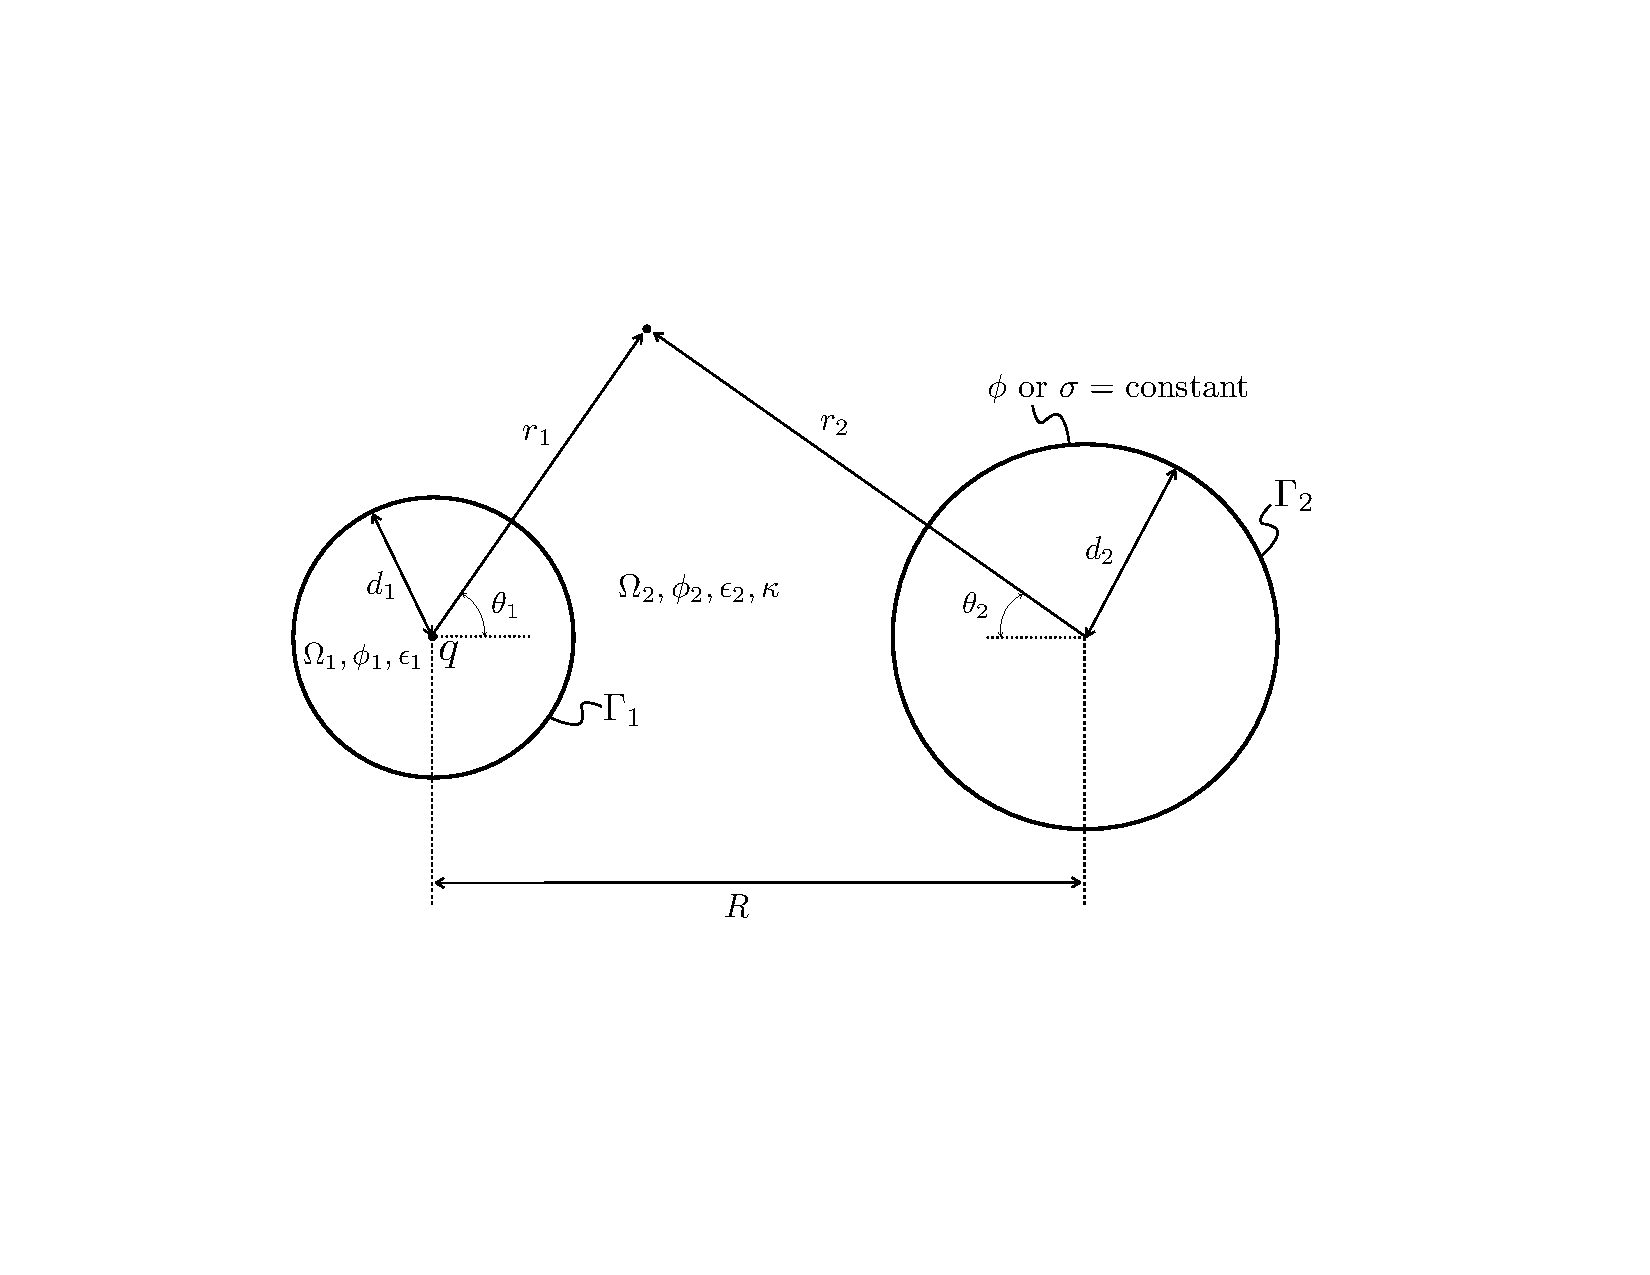
\includegraphics[width=0.45\textwidth]{Figure7.pdf} 
   \caption{Sketch of system solved with Legendre polynomials expansions.}
   \label{fig:twosphere_an}
\end{figure}
 

We make use of the following addition formula, \cite{MarceljaMitchellNinhamSculley1977}
%
\begin{equation} \label{eq:addition_formula}
k_n(\kappa r_2) P_n(\cos \theta_2) = \sum_{m=0}^{\infty}(2m+1) B_{nm} i_m(\kappa r_1) P_m(\cos \theta_1),
\end{equation}
%
\noindent to reformulate the expression for $\phi_2$ in Equation \eqref{eq:derivation1} as 
%
\begin{align} \label{eq:derivation2}
\phi_2 =& \sum_{n=0}^{\infty} a_n k_n(\kappa r_1) P_n(\cos \theta_1) \nonumber \\
& + \sum_{n=0}^{\infty} b_n \sum_{m=0}^{\infty}(2m+1) B_{nm} i_m(\kappa r_1) P_m(\cos \theta_1) \nonumber \\ 
\phi_2 =& \sum_{n=0}^{\infty} b_n k_n(\kappa r_2) P_n(\cos \theta_2) \nonumber \\
& + \sum_{n=0}^{\infty} a_n \sum_{m=0}^{\infty}(2m+1) B_{nm} i_m(\kappa r_2) P_m(\cos \theta_2).
\end{align}

Here, $i_m$ is the modified spherical Bessel function of the first kind; $B_{nm}$ is defined by 

\begin{equation} \label{eq:Bnm}
B_{nm} = \sum_{\nu=0}^{\infty} A_{nm}^{\nu} k_{n+m-2\nu}(\kappa R),
\end{equation}

\noindent where $R$ is the center-to-center distance; and $A_{nm}^{\nu}$ is given by the following expression, with ${\bf \Gamma}$ (in this context only) representing the gamma function:

%\begin{widetext}
\begin{equation} \label{eq:Anm}
A_{nm}^{\nu} = \frac{{\bf \Gamma}(n-\nu+0.5){\bf \Gamma}(m-\nu+0.5){\bf \Gamma}(\nu+0.5)(n+m-\nu)!(n+m-2\nu+0.5)}{\pi {\bf \Gamma}(m+n-\nu+1.5)(n-\nu)!(m-\nu)!\nu!}.
\end{equation}
%\end{widetext}



Legendre polynomials are orthogonal to each other, and $\frac{q}{4\pi\epsilon_1 r_1}$ is independent of $\theta$. Thus, taking the inner product of the expressions in Equations \eqref{eq:derivation1} and  \eqref{eq:derivation2} with $P_j(\cos \theta_i)$, where $i=1$ or $2$, yields
%
\begin{equation} \label{eq:derivation3}
\phi_1\delta_{0j} = c_j r_1^j + \frac{q}{4\pi\epsilon_1 r_1} \delta_{0j}  
\end{equation}
\noindent for the first expression of Equation \eqref{eq:derivation1}, and
%
\begin{align} \label{eq:derivation3.5}
\phi_2\delta_{0j} = &a_j k_j(\kappa r_1) + \sum_{n=0}^{\infty} b_n(2j+1)B_{nj} i_j(\kappa r_1),  \nonumber \\
\phi_2\delta_{0j} = &b_j k_j(\kappa r_2) + \sum_{n=0}^{\infty} a_n(2j+1)B_{nj} i_j(\kappa r_2)  
\end{align}
\noindent for Equation \eqref{eq:derivation2}.

Applying the interface conditions for $\Gamma_1$ on Equation \eqref{eq:derivation3} and the first expression of Equation \eqref{eq:derivation3.5}, produces
%
\begin{align}\label{eq:derivation4}
\sum_{n=0}^{\infty} a_n \left( \kappa k_{n}'(\kappa d_1) - \frac{\epsilon_1}{\epsilon_2} \frac{n}{d_1} k_n(\kappa d_1) \right) \delta_{nj} +& \nonumber \\ 
b_n (2j+1)B_{nj} \left( \kappa i_{j}'(\kappa d_1) - \frac{\epsilon_1}{\epsilon_2} \frac{j}{d_1} i_j(\kappa d_1)  \right) & = \nonumber \\
-\frac{\epsilon_1}{\epsilon_2} \frac{q}{4\pi\epsilon_1 d_1^2} \delta_{0j}&(j+1),
\end{align}

\noindent where $d_1$ is the radius of surface $1$.

\subsubsection*{Constant potential $\phi$ on $\Gamma_2$.}
The application of the boundary condition on $\Gamma_2$, $\phi(\Gamma_2) = \phi_0$, where $\phi_0$ is independent on $\theta_2$, gives

\begin{equation} \label{eq:derivation5_phi}
\sum_{n=0}^{\infty} a_n(2j+1)B_{nj}i_j(\kappa d_2) + b_nk_n(\kappa d_2) \delta_{nj} = \phi_0 \delta_{0j}.
\end{equation}

\noindent Combining Equations \eqref{eq:derivation4} and  \eqref{eq:derivation5_phi} yields the following system of equations for the coefficients $a_n$ and $b_n$
%
\begin{align} \label{eq:system_phi}
\mathbf{I} \mathbf{A} + \mathbf{L} \mathbf{B} &= -\frac{\epsilon_1}{\epsilon_2} \frac{q}{4\pi\epsilon_1 d_1^2} \mathbf{e} \nonumber \\
\mathbf{M} \mathbf{A} + \mathbf{I} \mathbf{B} &= \phi_0 \mathbf{e}
\end{align}

\noindent where
%
\begin{align} \label{eq:phi_terms}
I_{jn} &= \delta_{jn} \nonumber \\
e_j &= \delta_{0j} \nonumber \\
A_n &= a_n \left(\kappa k_n'(\kappa d_1) - \frac{\epsilon_1}{\epsilon_2} \frac{n}{d_1} k_n(\kappa d_1) \right) \nonumber \\
B_n &= b_n k_n(\kappa d_2) \nonumber \\
L_{jn} &= (2j+1)B_{nj}\left( \kappa \frac{i_j'(\kappa d_1)}{k_n(\kappa d_2)} - \frac{\epsilon_1}{\epsilon_2} \frac{j}{d_1} \frac{i_j(\kappa d_1)}{k_n(\kappa d_2)} \right) \nonumber \\
M_{jn} &= (2j+1)B_{nj} i_j(\kappa d_2) \frac{1}{\left(\kappa k_n'(\kappa d_1) - \frac{\epsilon_1}{\epsilon_2} \frac{n}{d_1} k_n(\kappa d_1) \right)}. 
\end{align}

\subsubsection*{Constant surface charge $\sigma$ on $\Gamma_2$.}
In this case, the application of the boundary condition on $\Gamma_2$, $\sigma(\Gamma_2) = -\epsilon_2 \frac{\partial \phi}{\partial \mathbf{n}} \Large|_{\Gamma_2} = \sigma_0$, where $\sigma_0$ is independent on $\theta_2$, gives

\begin{equation} \label{eq:derivation5_dphi}
\sum_{n=0}^{\infty} a_n(2j+1)B_{nj}\kappa i_j'(\kappa d_2) + b_n \kappa k_n'(\kappa d_2) \delta_{nj} = -\frac{\sigma_0}{\epsilon_2} \delta_{0j}
\end{equation}

\noindent Combining Equations \eqref{eq:derivation4} and  \eqref{eq:derivation5_phi} produces a system of equations for the coefficients $a_n$ and $b_n$
%
\begin{align} \label{eq:system_dphi}
\mathbf{I} \mathbf{A} + \mathbf{L} \mathbf{B} &= -\frac{\epsilon_1}{\epsilon_2} \frac{q}{4\pi\epsilon_1 d_1^2} \mathbf{e} \nonumber \\
\mathbf{M} \mathbf{A} + \mathbf{I} \mathbf{B} &= -\frac{\sigma_0}{\epsilon_2} \mathbf{e}
\end{align}

\noindent where
%
\begin{align} \label{eq:dphi_terms}
I_{jn} &= \delta_{jn} \nonumber \\
e_j &= \delta_{0j} \nonumber \\
A_n &= a_n \left(\kappa k_n'(\kappa d_1) - \frac{\epsilon_1}{\epsilon_2} \frac{n}{d_1} k_n(\kappa d_1) \right) \nonumber \\
B_n &= b_n \kappa k_n'(\kappa d_2) \nonumber \\
L_{jn} &= (2j+1)B_{nj}\left( \frac{i_j'(\kappa d_1)}{k_n'(\kappa d_2)} - \frac{\epsilon_1}{\epsilon_2} \frac{j}{d_1} \frac{i_j(\kappa d_1)}{\kappa k_n'(\kappa d_2)} \right) \nonumber \\
M_{jn} &= (2j+1)B_{nj} \kappa i_j'(\kappa d_2) \frac{1}{\left(\kappa k_n'(\kappa d_1) - \frac{\epsilon_1}{\epsilon_2} \frac{n}{d_1} k_n(\kappa d_1) \right)}. 
\end{align}
 
\subsection{Energy calculation} \label{energy_analytical}


 \medskip
 \paragraph*{Solvation free energy of the molecule---}
According to Equation \eqref{eq:solv_energy}, the solvation free energy of a molecule with a centered charge is given by
%
\begin{equation} \label{eq:energy_phi}
F_{\text{solv}} = \frac{1}{2} q \phi_{\text{reac}}(r_1=0),
\end{equation} 
 
 \noindent and using Equation \eqref{eq:derivation1}, the reaction potential from Equation \eqref{eq:phi_reac_bem} is:
 %
 \begin{equation} \label{eq:phi_reac_an}
 \phi_{\text{reac}} = \phi - \frac{q}{4\pi\epsilon_1 r} = \sum_{n=0}^{\infty} c_n r^n P_n(\cos \theta_1).
 \end{equation}
 
 Applying the boundary conditions at $\Gamma_1$ on Equation  \eqref{eq:derivation3}, we can rewrite $c_j$ in terms of the already computed $a_j$ and $b_j$:
 %
 \begin{align}
 c_j = \frac{1}{d_1^j} & \Big(a_j k_j(\kappa d_1) + \nonumber \\
&  \sum_{m=0}^{\infty} b_m(2j+1)B_{mj} i_j(\kappa d_1) - \frac{q}{4\pi\epsilon_1 d_1} \delta_{0j} \Big)
 \end{align} 
 
Because the charge is located at $r=0$, only the $n=0$ terms of Equation \eqref{eq:phi_reac_an} will survive, and the potential at this location is:
 
 \begin{align} \label{eq:phi_reac_an2}
 \phi_{\text{reac}} (r_1=0) = & a_0 k_0(\kappa d_1) + \nonumber \\
 &\sum_{m=0}^{\infty} b_m B_{m0}i_0(\kappa d_1) - \frac{q}{4\pi\epsilon_1 d_1}
 \end{align}
 
 The result from Equation \eqref{eq:phi_reac_an2} in Equation \eqref{eq:energy_phi} yields the solvation free energy. 
 
For the isolated molecule, $R \to \infty$ makes $B_{nm} \to 0$, which nullifies the sum in Equation \eqref{eq:phi_reac_an2} and $a_0$ for $R \to \infty$, from the system in Equation \eqref{eq:system_phi}, is 

\begin{equation} \label{eq:a0_inf}
a_0^{\infty} = -\frac{q}{d_1^2}\frac{\epsilon_1}{\epsilon_2} \frac{1}{4\pi\kappa k_0'(\kappa d_1) \epsilon_1}
\end{equation}


\medskip
\paragraph*{Surface  free energy with set potential $\phi_0$---}
We can expand $G_p$ from Equation \eqref{eq:energy_surf} in Legendre polynomials as
%
\begin{align} \label{eq:G_p}
G_p = &-\frac{\epsilon_2 \kappa}{\phi_0}  \Bigg[ \sum_{n=0}^{\infty} b_n k_n'(\kappa d_2) P_n(\cos \theta_2) \nonumber \\ 
& + \sum_{n=0}^{\infty} a_n \sum_{m=0}^{\infty} (2m+1) B_{nm} i_m'(\kappa d_2) P_m(\cos \theta_2) \Bigg].
\end{align}

 \noindent Applying Equation \eqref{eq:G_p} in Equation \eqref{eq:energy_surf} gives

\begin{equation} \label{G_p_int}
F = 2\pi \kappa \phi_0 d_2^2 \epsilon_2 \left[ b_0 k_0'(\kappa d_2) + \sum_{n=0}^{\infty} a_n B_{n0} i_0'(\kappa d_2) \right]
\end{equation}

 \noindent If the surface is isolated, $R \to \infty$ makes $B_{n0} \to 0$, and the free energy in this case is 
%
\begin{equation} \label{energy_isolated_phi}
F = 2\pi \kappa \phi_0 d_2^2 b_0^{\infty} k_0'(\kappa d_2) \epsilon_2
\end{equation}
 
 \noindent where $b_0^{\infty}$ is taken from the system in  \eqref{eq:system_phi} considering $B_{nm} \to 0$, which results in
 %
 \begin{equation} \label{b_inf_phi}
 b_0^{\infty} = \frac{\phi_0}{k_0(\kappa d_2)}.
 \end{equation}
 
 \medskip
 \paragraph*{Surface  free energy with set charge $\sigma_0$---}
We can expand $G_c$ from Equation \eqref{eq:energy_surf} in Legendre polynomials as
%
\begin{align} \label{eq:G_c}
G_c = & \frac{1}{\sigma_0} \Bigg[ \sum_{n=0}^{\infty} b_n k_n(\kappa d_2) P_n(\cos \theta_2) + \nonumber \\ 
&\sum_{n=0}^{\infty} a_n \sum_{m=0}^{\infty} (2m+1) B_{nm} i_m(\kappa d_2) P_m(\cos \theta_2) \Bigg]
\end{align}

 \noindent Applying Equation \eqref{eq:G_c} into Equation \eqref{eq:energy_surf} gives

\begin{equation} \label{G_c_int}
F = 2\pi \sigma_0 d_2^2 \left[ b_0 k_0(\kappa d_2) + \sum_{n=0}^{\infty} a_n B_{n0} i_0(\kappa d_2) \right]
\end{equation}

 \noindent For the isolated surface, $R \to \infty$ and $B_{n0} \to 0$, and the free energy is 
%
\begin{equation} \label{energy_isolated_dphi}
F = 2\pi \sigma_0 d_2^2 b_0^{\infty} k_0(\kappa d_2) 
\end{equation}
 
 \noindent where $b_0^{\infty}$ is calculated from the system in  \eqref{eq:system_dphi} considering $B_{nm} \to 0$, which results in
 
 \begin{equation} \label{b_inf_dphi}
 b_0^{\infty} = -\frac{\sigma_0}{\epsilon_2 \kappa k_0'(\kappa d_2)}.
 \end{equation}


\section{Results of the grid-convergence study} \label{sec:results}
%!TEX root = CooperBarba2014.tex

The results detailed in this section were obtained using an extension of the open source code \pygbe,\footnote{\url{https://github.com/barbagroup/pygbe}} that accounts for the presence of surfaces with imposed charge or potential.\cite{CooperBarba2015a}
We performed the calculations for protein G B1 D4$^\prime$ on a workstation with Intel Xeon X5650 \cpu s  and one \nvidia Tesla C2075 \gpu\ card. 
The final case considers the antibody immunoglobulin G, which is a much larger molecule than protein G. For these runs, we used Boston University's \textsc{bungee} cluster, which has 16 nodes with 8 Intel Xeon \cpu\ cores each, and a total of 3 \nvidia Tesla Kepler K20 and 26 \nvidia Tesla M2070/2075 \gpu s. All runs were serial: single-\cpu\ and single-\gpu. 
We obtained the van der Waals radii and charge distribution using \texttt{pdb2pqr}\cite{Dolinsky04} with an \amber forcefield, and generated the meshes using the free \msms software.\cite{SannerOlsonSpehner1995}
In these tests, we did not consider a Stern layer for either the protein or the charged surface, nor the presence of solvent-filled cavities inside the protein.

\subsection{First case: protein G B1 D4$^{\prime}$} \label{sec:PGB}

We computed the electrostatic field of protein G B1 D4$^{\prime}$ interacting with a 100\AA$\times$100\AA$\times$10\AA\ block with surface charge density $\pm$0.05C/m$^2$, and investigated its preferred orientation. The protein was centered with respect to a  100\AA$\times$100\AA\ face, a distance 2\AA\ above it. 
As seen in Figure \ref{fig:1pgb_orientation}, $\alpha_\text{tilt}$ is the angle between the protein's dipole moment and the normal vector to the surface, and $\alpha_\text{rot}$ rotates about the dipole moment. The dipole-moment vector placed at the center of mass of the protein generates an axis, and we used the line of shortest distance between the outermost atom and this axis as a reference vector $\mathbf{V}_{\text{ref}}$. The rotation angle $\alpha_{\text{rot}}$ is the angle between the normal vector to a 100\AA$\times$10\AA\ side face of the block and $\mathbf{V}_{\text{ref}}$.

In these cases, we considered a solvent with no salt, i.e., $\kappa=0$ (to compare with other published results), and with relative permittivity 80. The region inside the protein had a relative permittivity of 4.

\medskip

 \paragraph*{Grid-convergence study for protein G B1 D4$^{\prime}$---}

By means of a grid-convergence study, we make sure that the runs are in the asymptotic range of the model, select a triangle density so that the geometry is well-resolved by the surface mesh, and find adequate values of the simulation parameters for sampling the orientations. Using Richardson extrapolation, we find values of the energy that estimate the exact solution and use them as a reference to calculate estimated errors. This error is simply the relative difference between the energy obtained numerically with each mesh density and the estimated exact value. In this way, we choose the parameters for the sampling runs with confidence that they are both accurate and efficient in computing time. 

We computed the solvation and surface energy of a system containing a surface with charge density 0.05C/m$^2$, and a protein at $\alpha_{\text{tilt}} = 10^{\circ}$ and $\alpha_{\text{rot}} = 200^{\circ}$. The numerical parameters are presented in Table \ref{table:params2}. Using runs with mesh densities of 2, 4, and 8 elements per square Angstrom, we obtained the values in Table \ref{table:extraPGB} using Richardson extrapolation: these are the reference values for the error plotted in Figure \ref{fig:convergence_1PGB_sensor}. The observed order of convergence was 0.96 for the solvation energy and 0.94 for the surface energy. For details on the Richardson-extrapolation method for performing grid-convergence analysis, see our previous work.\cite{CooperBardhanBarba2013} 
Figure \ref{fig:convergence_1PGB_sensor} shows errors that are decaying as $1/N$ in both the solvation and surface energies for the finest three meshes. This indicates that the calculations are in the asymptotic region and the geometry is well resolved in these cases.

\begin{table}[h]
  %\centering
   %\fontfamily{ppl}\selectfont
   \caption{\label{table:params2}Numerical parameters used in the convergence runs with protein G B1 D4$^{\prime}$. } 
    \begin{tabular}{c c c c c c c}
	\hline%\toprule
	\multicolumn{3}{l} {\# Gauss points:} & \multicolumn{3}{l}{Treecode:} & \gmres:\\
	\footnotesize{in-element} & \footnotesize{close-by} & \footnotesize{far-away} & $N_{\text{crit}}$ & $P$ &  $\theta$  & tol.\\
	\hline%\midrule
	9 per side & 19 & 7  &  500 & 15 & 0.5  & $10^{-8}$\\	
	\hline%\bottomrule
    \end{tabular}
\end{table}



\begin{table}[h]
  %\centering
   %\fontfamily{ppl}\selectfont
   \caption{\label{table:extraPGB}Extrapolated values of energy for protein G B1 D4$^\prime$.} 
    \begin{tabular}{c c}
	\hline%\toprule
	\multicolumn{2}{c} {Energy [kcal/mol]} \\
	Solvation & Surface \\
	\hline%\midrule
	$-222.43$ & $317.98$ \\	
	\hline%\bottomrule
    \end{tabular}
\end{table}

\begin{figure}[h] %  figure placement: here, top, bottom, or page
   \centering
   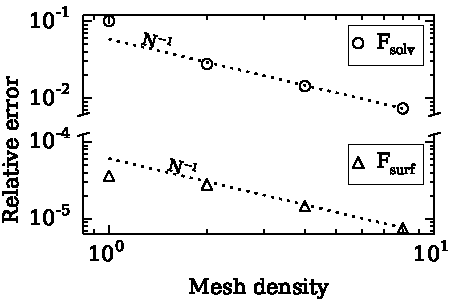
\includegraphics[width=0.45\textwidth]{Figure10.pdf} 
   \caption{Grid-convergence study of the solvation and surface energy for protein G B1 D4$^{\prime}$ mutant, interacting with a surface with a charge density of 0.05C/m$^2$. Data sets, figure files and running/plotting scripts available under \ccby.\cite{CooperBarba2015-share1348803}}
   \label{fig:convergence_1PGB_sensor}
\end{figure}



\medskip

 \paragraph*{Probing orientation of Protein G B1 D4$^{\prime}$---}

We sampled the total free energy every $\Delta \alpha_{\text{tilt}} = 2^\circ$ of tilt angle and $\Delta \alpha_{\text{rot}} =10^\circ$ of rotation angle, resulting in $3,240$ independent runs.  The surface mesh had 4 triangles per square Angstrom on the protein geometry and 2 triangles per square Angstrom on the charged surface. Numerical parameters are presented in Table \ref{table:params3}.

\begin{table}[h]
  %\centering
   %\fontfamily{ppl}\selectfont
   \caption{\label{table:params3}Numerical parameters used in the runs probing orientation of protein G B1 D4$^{\prime}$. } 
    \begin{tabular}{c c c c c c c}
	\hline%\toprule
	\multicolumn{3}{l} {\# Gauss points:} & \multicolumn{3}{l}{Treecode:} & \gmres:\\
	\footnotesize{in-element} & \footnotesize{close-by} & \footnotesize{far-away} & $N_{\text{crit}}$ & $P$ &  $\theta$  & tol.\\
	\hline%\midrule
	9 per side & 19 & 1  &  300 & 4 & 0.5  & $10^{-5}$\\	
	\hline%\bottomrule
    \end{tabular}
\end{table}

 

With total free energy as the input, the integrals of Equation \eqref{eq:prob_angle} can be computed by means of the trapezoidal rule. Figure \ref{fig:1PGB_probability} presents the probability of the protein orientation in terms of $\cos(\alpha_{\text{tilt}})$, in intervals of $\Delta \cos(\alpha_{\text{tilt}}) = 0.005$ (Fig.~\ref{fig:1PGB_cos}) and $\Delta \alpha_{\text{tilt}}$=2$^{\circ}$ (Fig.~\ref{fig:1PGB_alpha}. Table \ref{table:avg} presents the average orientation $<\cos(\alpha_{\text{tilt}})>$ for the surface having either positive or negative charge density, and Figure \ref{fig:field} shows the electrostatic potential for the preferred orientation in each case. 

\begin{figure*}
   \centering
   \subfloat[]{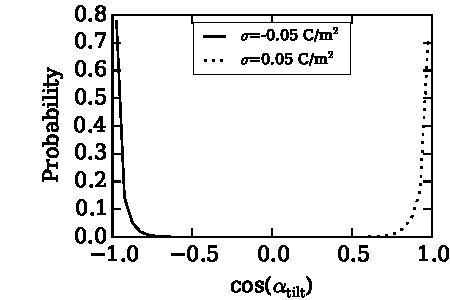
\includegraphics[width=0.43\textwidth]{Figure11a.pdf} \label{fig:1PGB_cos}}
   \subfloat[]{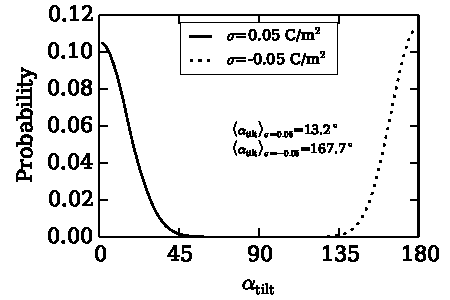
\includegraphics[width=0.43\textwidth]{Figure11b.pdf} \label{fig:1PGB_alpha}}\\
   \subfloat[]{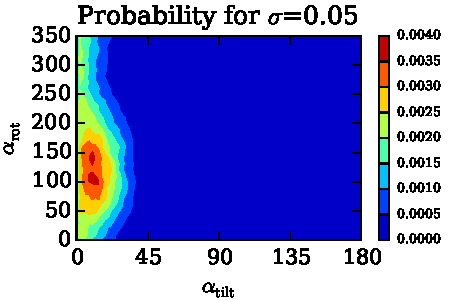
\includegraphics[width=0.40\textwidth]{Figure11c.pdf} \label{fig:1PGB_2D_sig005}}
   \subfloat[]{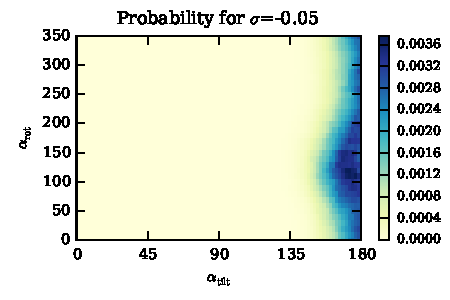
\includegraphics[width=0.40\textwidth]{Figure11d.pdf} \label{fig:1PGB_2D_sig-005}}
   \caption{Orientation probability distribution of protein G B1 D4$^{\prime}$. Figures \ref{fig:1PGB_cos} and \ref{fig:1PGB_alpha} are the probability with respect to the tilt angle and its cosine, respectively. Figures \ref{fig:1PGB_2D_sig005} and \ref{fig:1PGB_2D_sig-005} are the probability with respect to both the tilt and rotation angle. Data sets, figure files and running/plotting scripts available under \ccby.\cite{CooperBarba2015-share1348804}}
   \label{fig:1PGB_probability}
\end{figure*}

\begin{table}[h]
   \caption{\label{table:avg}Average orientation.} 
    \begin{tabular}{c c}
	\hline
	\multicolumn{2}{c} {$<\cos(\alpha_{\text{tilt}})>$} \\
	Negative & Positive \\
	\hline
	$-0.968$ & $0.963$ \\	
	\hline
    \end{tabular}
\end{table}

\begin{figure*}
   \centering
   \subfloat[Negative surface charge ($\alpha_\text{tilt}=172^\circ$, $\alpha_\text{rot}=110^\circ$)]{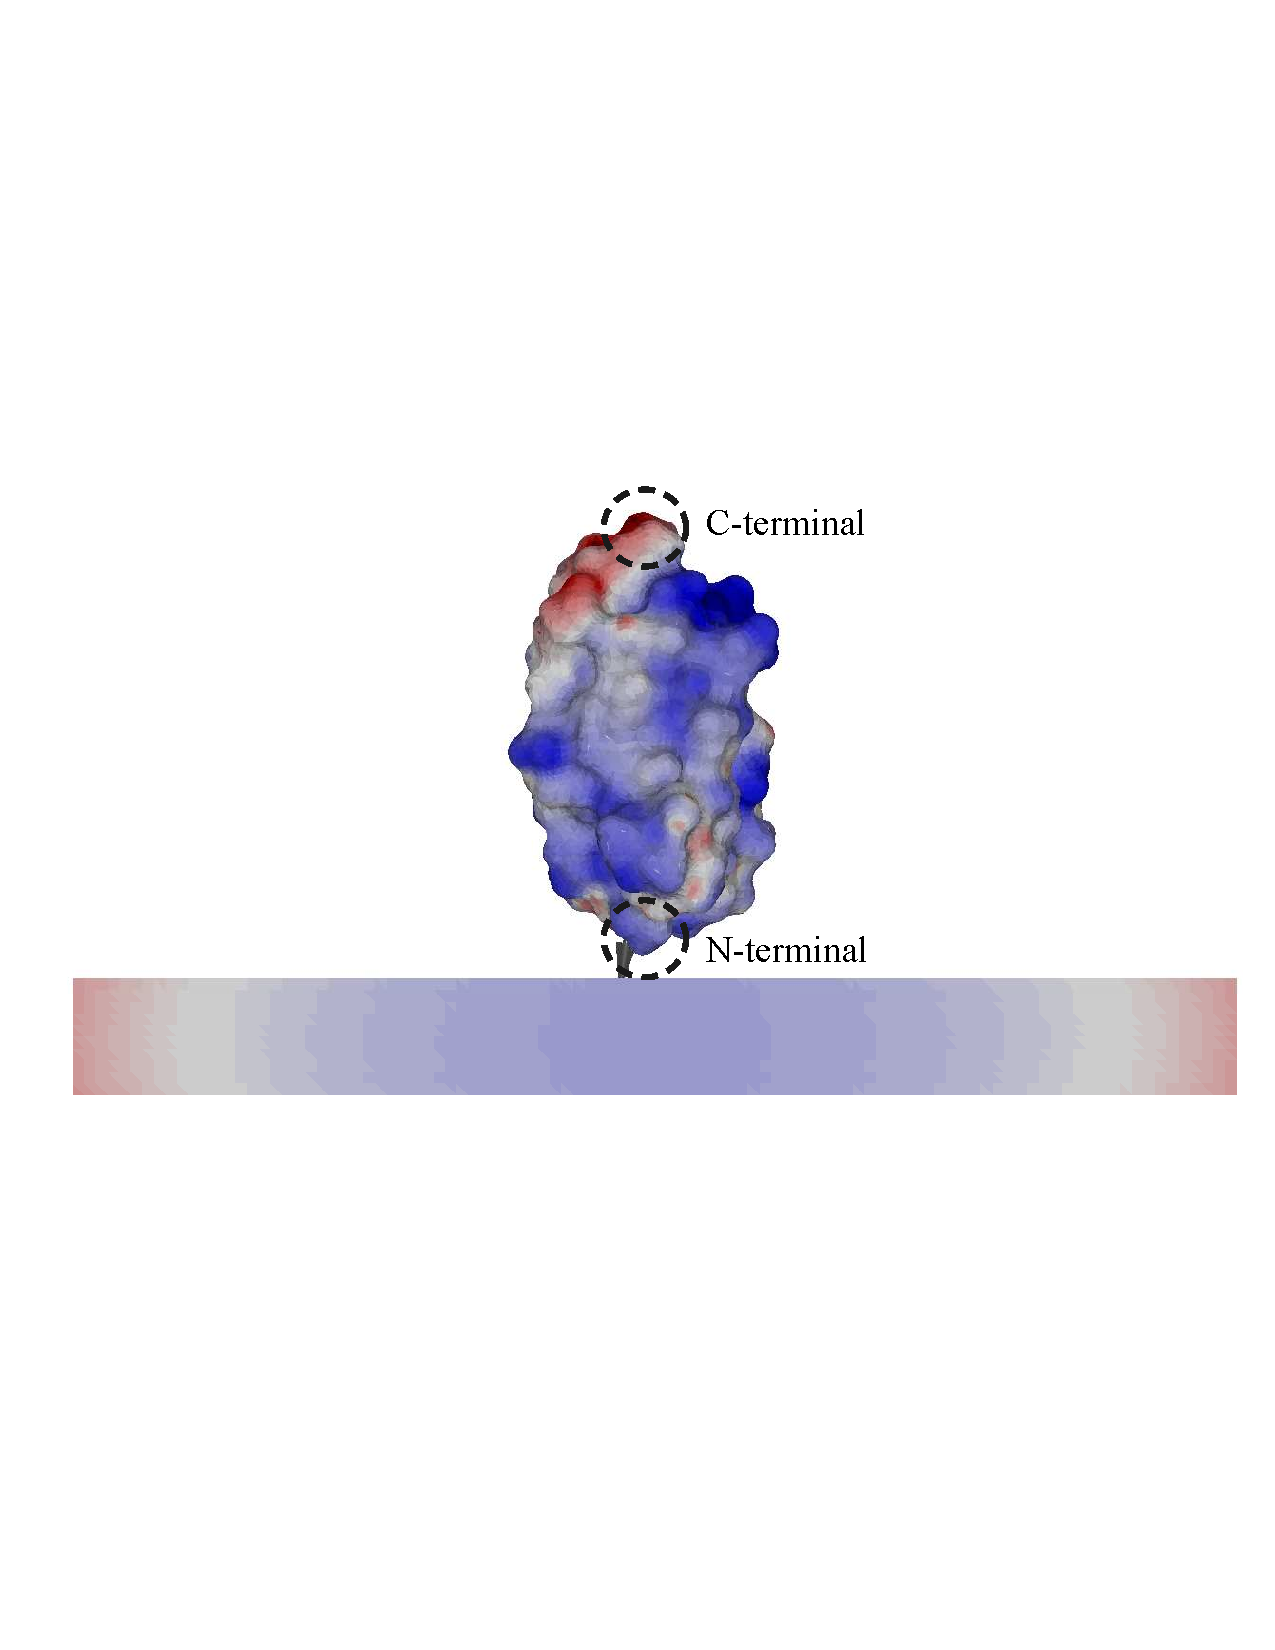
\includegraphics[width=0.48\textwidth]{Figure12a.pdf} \label{fig:phi_sig-0.05}} 
   %\subfloat[Surface charge density with negative surface charge]{\includegraphics[width=0.5\textwidth]{dphi_sig-005.pdf} \label{fig:dphi_sig-0.05}} \\
   \subfloat[Positive surface charge ($\alpha_\text{tilt}=8^\circ$, $\alpha_\text{rot}=150^\circ$)]{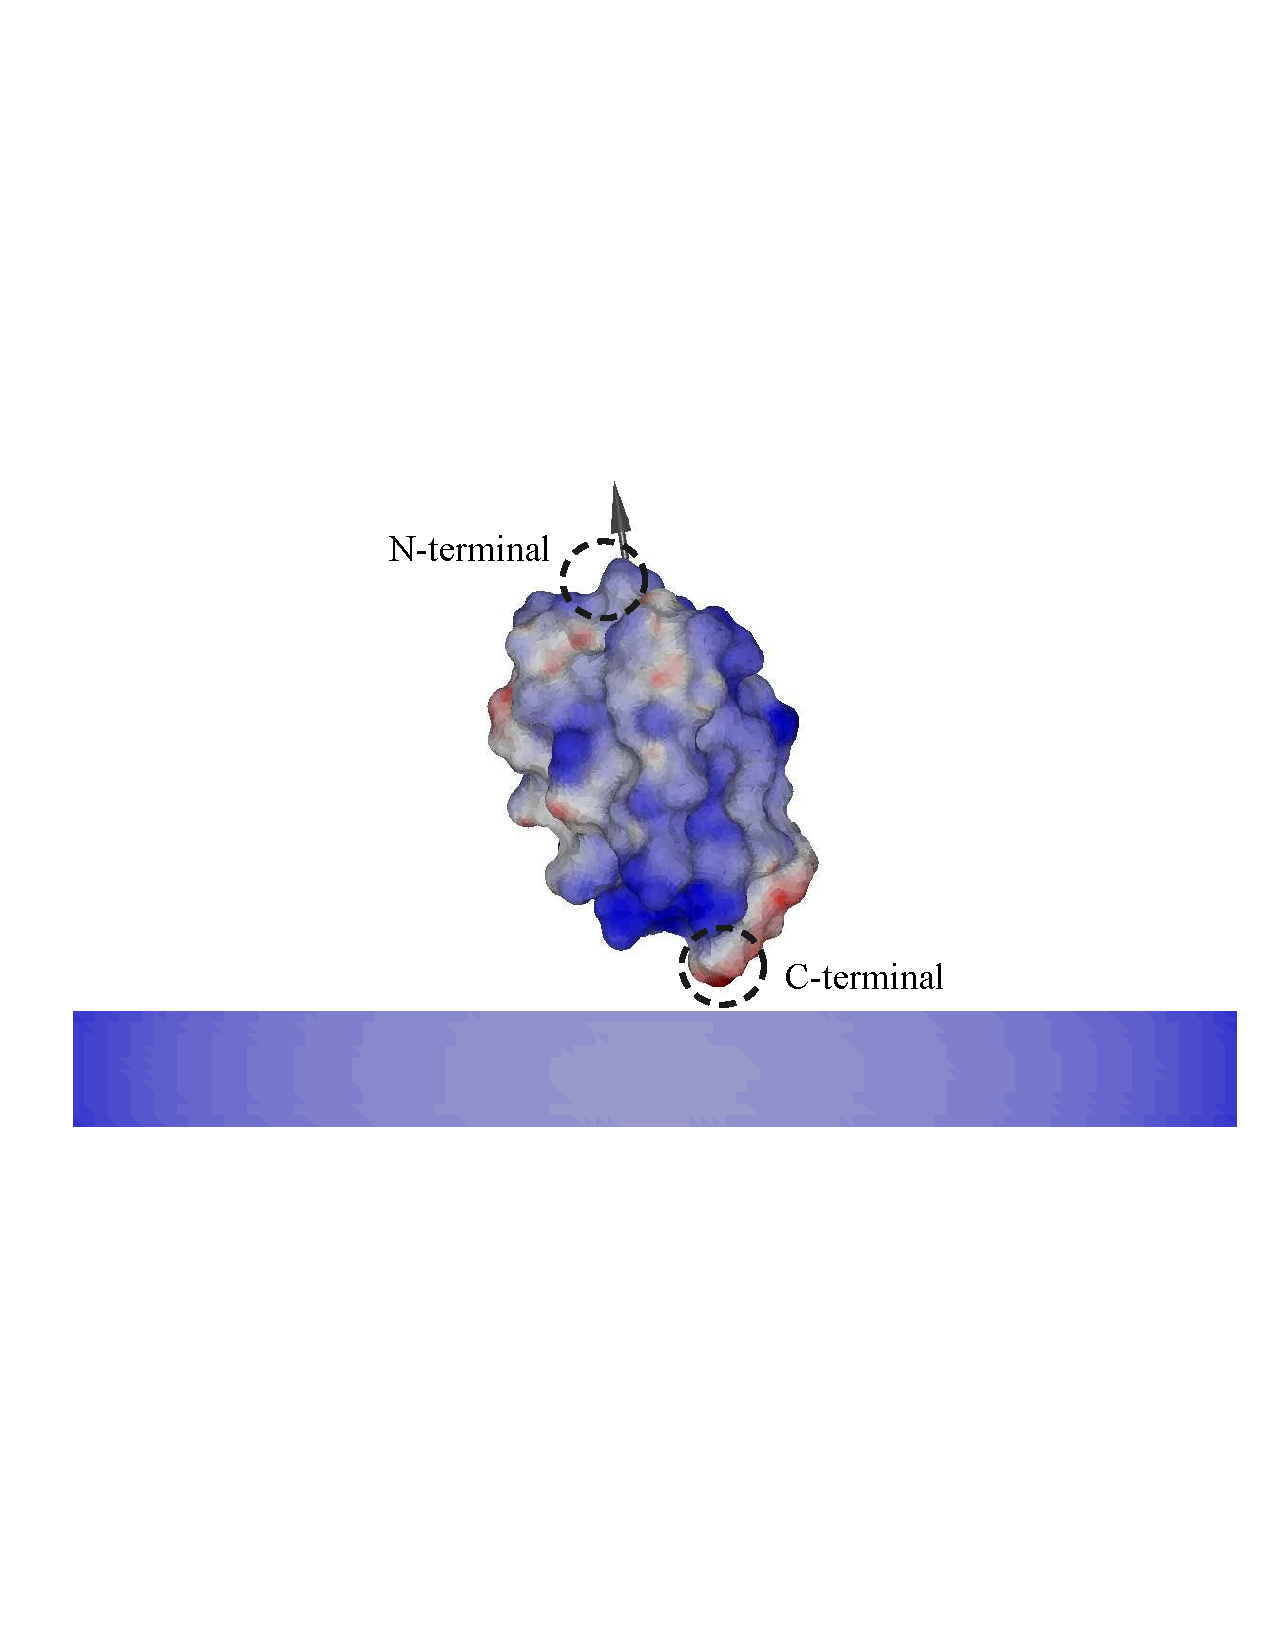
\includegraphics[width=0.48\textwidth]{Figure12b.pdf} \label{fig:phi_sig0.05}} 
   %\subfloat[Surface charge density with positive surface charge]{\includegraphics[width=0.5\textwidth]{dphi_sig005.pdf} \label{fig:dphi_sig0.05}}
   \caption{Electrostatic potential of protein G B1 D4$^{\prime}$ for the preferred orientations according to Figure \ref{fig:1PGB_probability}. Black arrow indicates direction of dipole-moment vector.}
   \label{fig:field}
\end{figure*}

\subsection{Second case: immunoglobulin G} \label{sec:IGT}


We computed the electrostatic field of immunoglobulin G---a protein widely used in biosensors---interacting with a 250\AA$\times$250\AA$\times$10\AA\ block, varying the conditions of surface charge and salt concentration. The protein was centered with respect to a  250\AA$\times$250\AA\ face, at a distance 5\AA\ above it. The solvent had relative permittivity of 80 and the protein of 4.

\medskip

 \paragraph*{Grid-convergence study for immunoglobulin G---}

As in the previous section, we carried out a grid-convergence study to make sure the geometry was well resolved and to find adequate values of the simulation parameters for sampling different orientations. The error in Figure \ref{fig:1IGT_convergence} is the relative difference between the energy obtained using \pygbe with each mesh density and the estimated exact value computed with Richardson extrapolation.

In this case, we computed the solvation energy and surface energy of a system consisting of a surface with charge density 0.05C/m$^2$ and a protein with $\alpha_{\text{tilt}} = 31^{\circ}$ and $\alpha_{\text{rot}} = 130^{\circ}$. Using the results from runs with a mesh density of 2, 4, and 8 elements per square Angstrom, we added the solvation and surface energies, and used Richardson extrapolation to obtain a value of $-2792.22$kcal/mol, and an \emph{observed order of convergence} of 0.85. This is our reference to calculate the errors in Figure \ref{fig:1IGT_convergence}. There is a slight deviation from the expected value of the observed order of convergence (1.0), which we attribute to the non-uniform mesh generated by \msms. Even though the mesh density is on average doubled for each run, there is no guarantee that the refinement is homogeneous throughout the whole molecular surface. The numerical parameters are presented in Table \ref{table:params4}.

\begin{table}[h]
  %\centering
   %\fontfamily{ppl}\selectfont
   \caption{\label{table:params4}Numerical parameters used in the convergence runs with immunoglobulin G. } 
    \begin{tabular}{c c c c c c c}
	\hline%\toprule
	\multicolumn{3}{l} {\# Gauss points:} & \multicolumn{3}{l}{Treecode:} & \gmres:\\
	\footnotesize{in-element} & \footnotesize{close-by} & \footnotesize{far-away} & $N_{\text{crit}}$ & $P$ &  $\theta$  & tol.\\
	\hline%\midrule
	9 per side & 19 & 1  &  1000 & 6 & 0.5  & $10^{-5}$\\	
	\hline%\bottomrule
    \end{tabular}
\end{table}




\begin{figure}[h] %  figure placement: here, top, bottom, or page
   \centering
   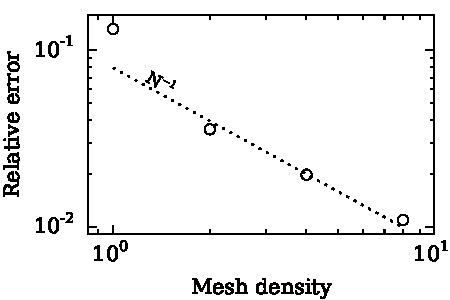
\includegraphics[width=0.45\textwidth]{Figure13.pdf} 
   \caption{Grid-convergence study of the solvation plus surface energy for immunoglobulin G interacting with a surface with charge density 0.05C/m$^2$. Data sets, figure files and plotting scripts available under \ccby.\cite{CooperBarba2015-share1348801}}
   \label{fig:1IGT_convergence}
\end{figure}



\medskip 

 \paragraph*{Probing orientation of immunoglobulin G---}

We sampled the total free energy every $\Delta \alpha_{\text{tilt}} = 4^\circ$ of tilt angle and $\Delta \alpha_{\text{rot}} =20^\circ$ of rotation angle, resulting in a total of 810 runs.  The surface meshes had 2 triangles per square Angstrom throughout. Numerical parameters are presented in Table \ref{table:params5}.

\begin{table}[h]
  %\centering
   %\fontfamily{ppl}\selectfont
   \caption{\label{table:params5}Numerical parameters used in the runs probing orientation of immunoglobulin G. } 
    \begin{tabular}{c c c c c c c}
	\hline%\toprule
	\multicolumn{3}{l} {\# Gauss points:} & \multicolumn{3}{l}{Treecode:} & \gmres:\\
	\footnotesize{in-element} & \footnotesize{close-by} & \footnotesize{far-away} & $N_{\text{crit}}$ & $P$ &  $\theta$  & tol.\\
	\hline%\midrule
	9 per side & 19 & 1  &  300 & 2 & 0.5  & $10^{-4}$\\	
	\hline%\bottomrule
    \end{tabular}
\end{table}

With the computed total free energy, we obtained the probability of each orientation using Equation \eqref{eq:prob_angle} and the trapezoidal rule. %Figure \ref{fig:probability} shows the probability of the protein orientation in terms of $\cos(\alpha_{\text{tilt}})$, in intervals of $\Delta \cos(\alpha_{\text{tilt}}) = 0.05$ for Figure \ref{fig:1IGT_cos}, and $\Delta \alpha_{\text{tilt}}$=4$^{\circ}$ for Figure \ref{fig:1IGT_alpha}.  
We sampled all combinations with surface charges of $\sigma=\pm$0.05C/m$^2$ and $\sigma = \pm$ 0.2C/m$^2$ and salt concentrations of 145mM ($\kappa$ = 0.125 \AA$^{-1}$) and 9mM ($\kappa$ = 0.03125 \AA$^{-1}$). For each of these cases, Figures \ref{fig:1IGT_negcharge}  and \ref{fig:1IGT_poscharge} show a color plot of the probability distribution with respect to the tilt and rotation angles, and a 3D plot of the preferred orientation, where the solvent-excluded surface is colored by the electrostatic potential.

\begin{figure*}
   \centering
   \subfloat[Probability for $\sigma$=-0.05C/m$^2$ and $\kappa$=0.125\AA$^{-1}$]{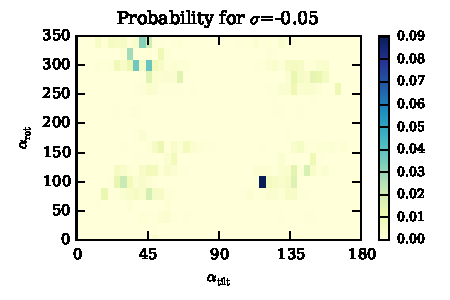
\includegraphics[width=0.4\textwidth]{Figure14a.pdf} \label{fig:1IGT_2D_sig-005}}
   \subfloat[Side view for $\alpha_{\text{tilt}} = 116^{\circ}$ and $\alpha_{\text{rot}} = 100^{\circ}$]{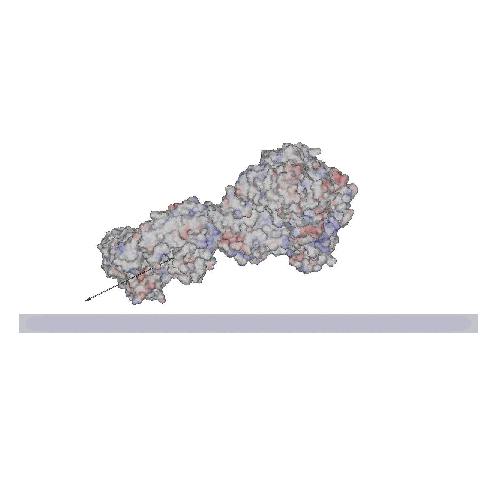
\includegraphics[width=0.4\textwidth]{Figure14b.pdf} \label{fig:1IGT_3D_sig-005_kap0125_til116-rot100}}\\
   \subfloat[Probability for $\sigma$=-0.2C/m$^2$ and $\kappa$=0.125\AA$^{-1}$]{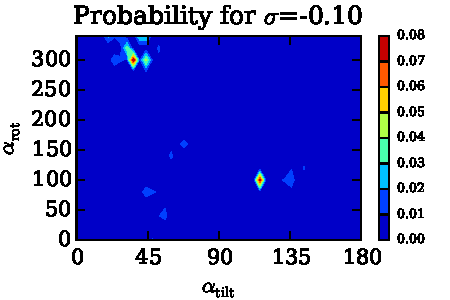
\includegraphics[width=0.4\textwidth]{Figure14c.pdf} \label{fig:1IGT_2D_sig-020_kappa01250}}
   \subfloat[Side view for $\alpha_{\text{tilt}} = 56^{\circ}$ and $\alpha_{\text{rot}} = 40^{\circ}$]{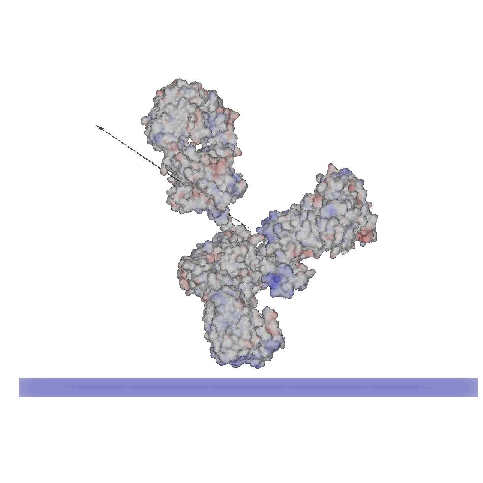
\includegraphics[width=0.4\textwidth]{Figure14d.pdf} \label{fig:1IGT_3D_sig-02_kap0125_til056-rot040}}\\
   \subfloat[Probability for $\sigma$=-0.05C/m$^2$ and $\kappa$=0.03125\AA$^{-1}$]{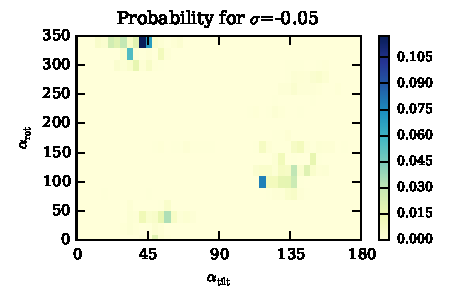
\includegraphics[width=0.4\textwidth]{Figure14e.pdf} \label{fig:1IGT_2D_sig-005_kappa003125}}
   \subfloat[Side view for $\alpha_{\text{tilt}} = 116^{\circ}$ and $\alpha_{\text{rot}} = 160^{\circ}$]{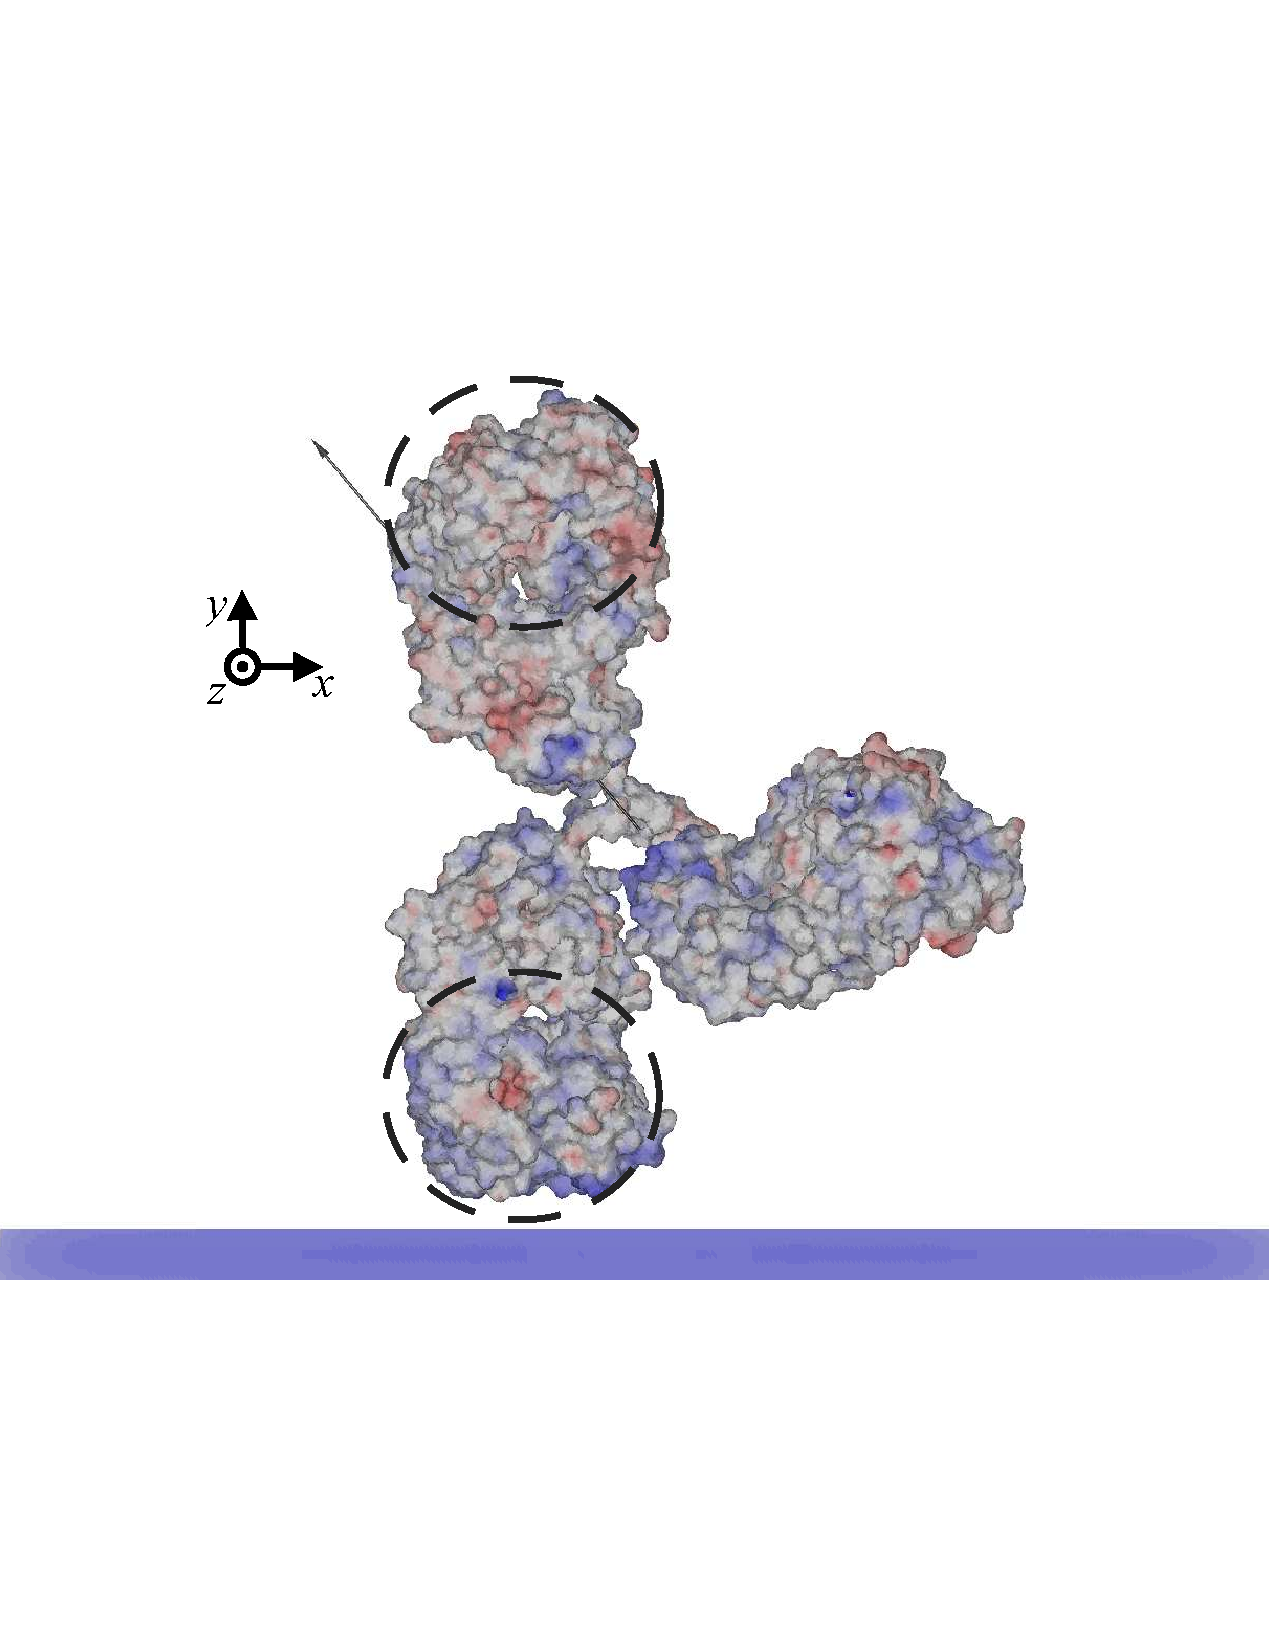
\includegraphics[width=0.4\textwidth]{Figure14f.pdf} \label{fig:1IGT_3D_sig-005_kap003125_til116-rot160}}\\
   \subfloat[Probability for $\sigma$=-0.2C/m$^2$ and $\kappa$=0.03125\AA$^{-1}$]{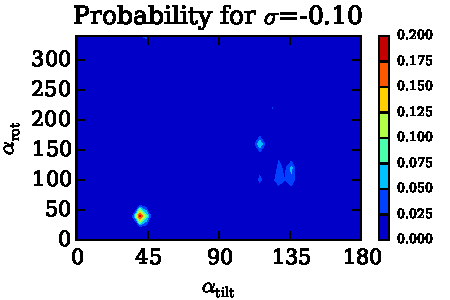
\includegraphics[width=0.4\textwidth]{Figure14g.pdf} \label{fig:1IGT_2D_sig-020_kappa003125}}
   \subfloat[Side view for $\alpha_{\text{tilt}} = 124^{\circ}$ and $\alpha_{\text{rot}} = 140^{\circ}$]{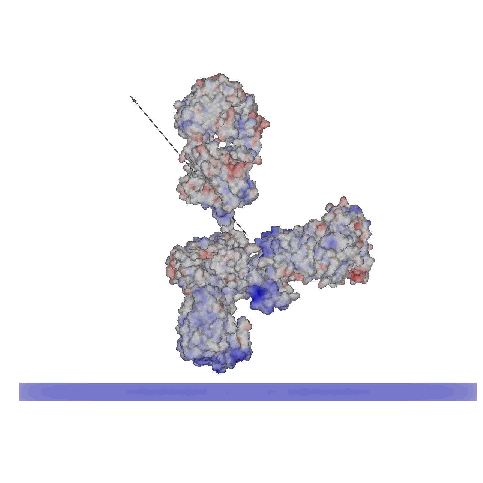
\includegraphics[width=0.4\textwidth]{Figure14h.pdf} \label{fig:1IGT_3D_sig-02_kap003125_til124-rot140}}
   \caption{Orientation probability distribution and surface potential of the preferred orientation for immunoglobulin G near a negative surface charge. The black arrow indicates the direction of the dipole moment. Data sets, figure files and plotting scripts available under \ccby.\cite{CooperBarba2015-share1348801}}
   \label{fig:1IGT_negcharge}
\end{figure*}


\begin{figure*}
   \centering
   \subfloat[Probability for $\sigma$=0.05C/m$^2$ and $\kappa$=0.125\AA$^{-1}$]{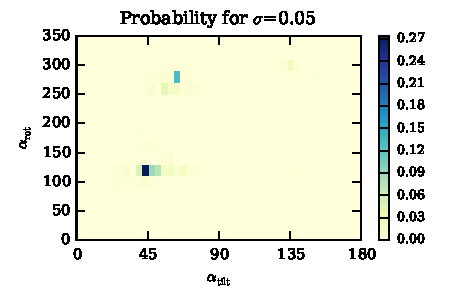
\includegraphics[width=0.4\textwidth]{Figure15a.pdf} \label{fig:1IGT_2D_sig005}}
   \subfloat[Side view for $\alpha_{\text{tilt}} = 64^{\circ}$ and $\alpha_{\text{rot}} = 280^{\circ}$]{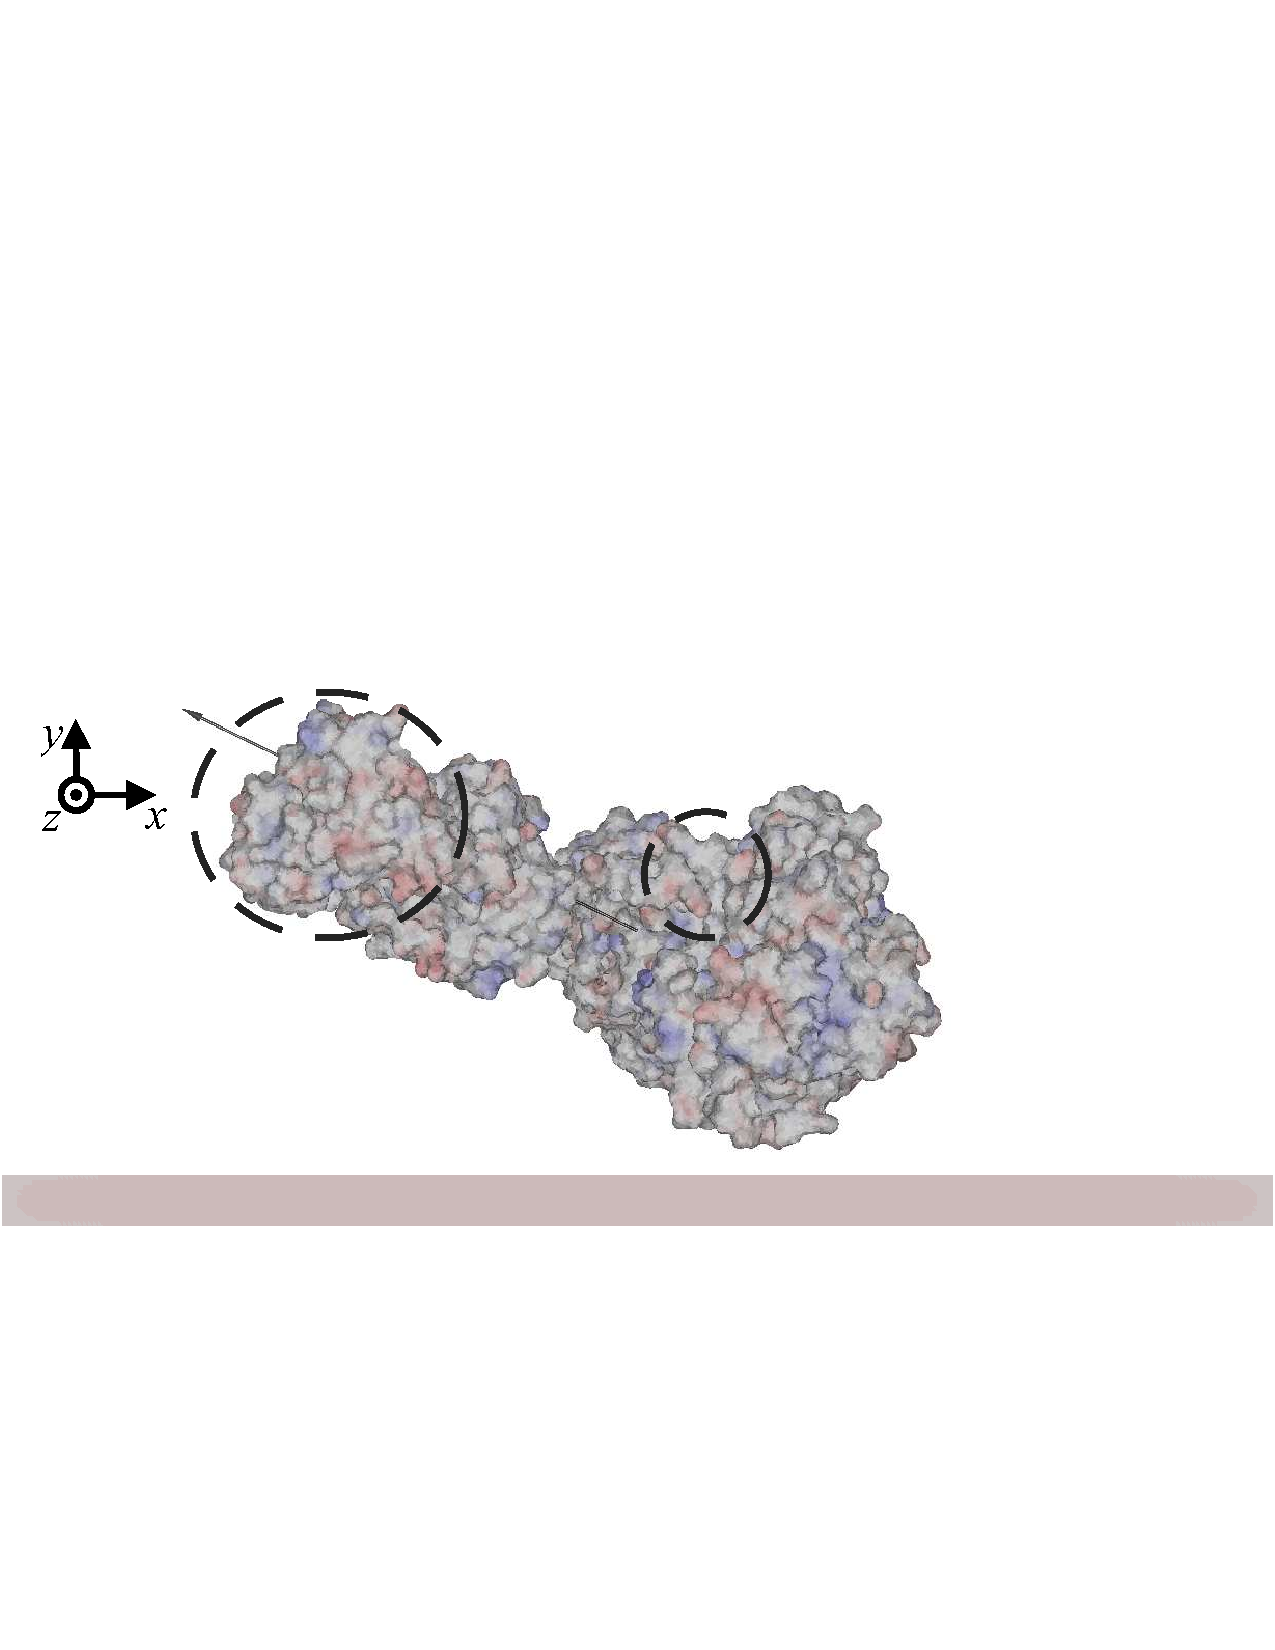
\includegraphics[width=0.4\textwidth]{Figure15b.pdf} \label{fig:1IGT_3D_sig005_kap0125_til064-rot280}}\\
   \subfloat[Probability for $\sigma$=0.2C/m$^2$ and $\kappa$=0.125\AA$^{-1}$]{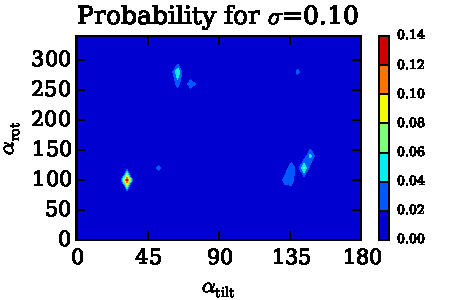
\includegraphics[width=0.4\textwidth]{Figure15c.pdf} \label{fig:1IGT_2D_sig020_kappa01250}}
   \subfloat[Side view for $\alpha_{\text{tilt}} = 64^{\circ}$ and $\alpha_{\text{rot}} = 260^{\circ}$]{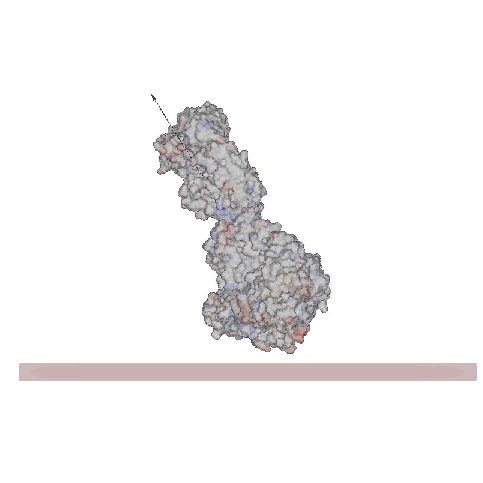
\includegraphics[width=0.4\textwidth]{Figure15d.pdf} \label{fig:1IGT_3D_sig02_kap0125_til064-rot260}}\\
   \subfloat[Probability for $\sigma$=0.05C/m$^2$ and $\kappa$=0.03125\AA$^{-1}$]{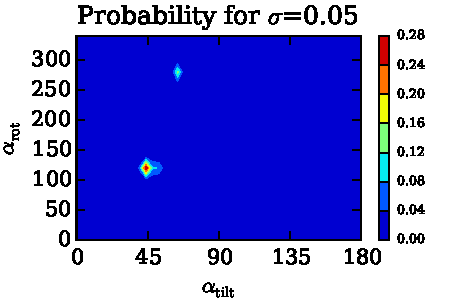
\includegraphics[width=0.4\textwidth]{Figure15e.pdf} \label{fig:1IGT_2D_sig005_kappa003125}}
   \subfloat[Side view for $\alpha_{\text{tilt}} = 44^{\circ}$ and $\alpha_{\text{rot}} = 120^{\circ}$]{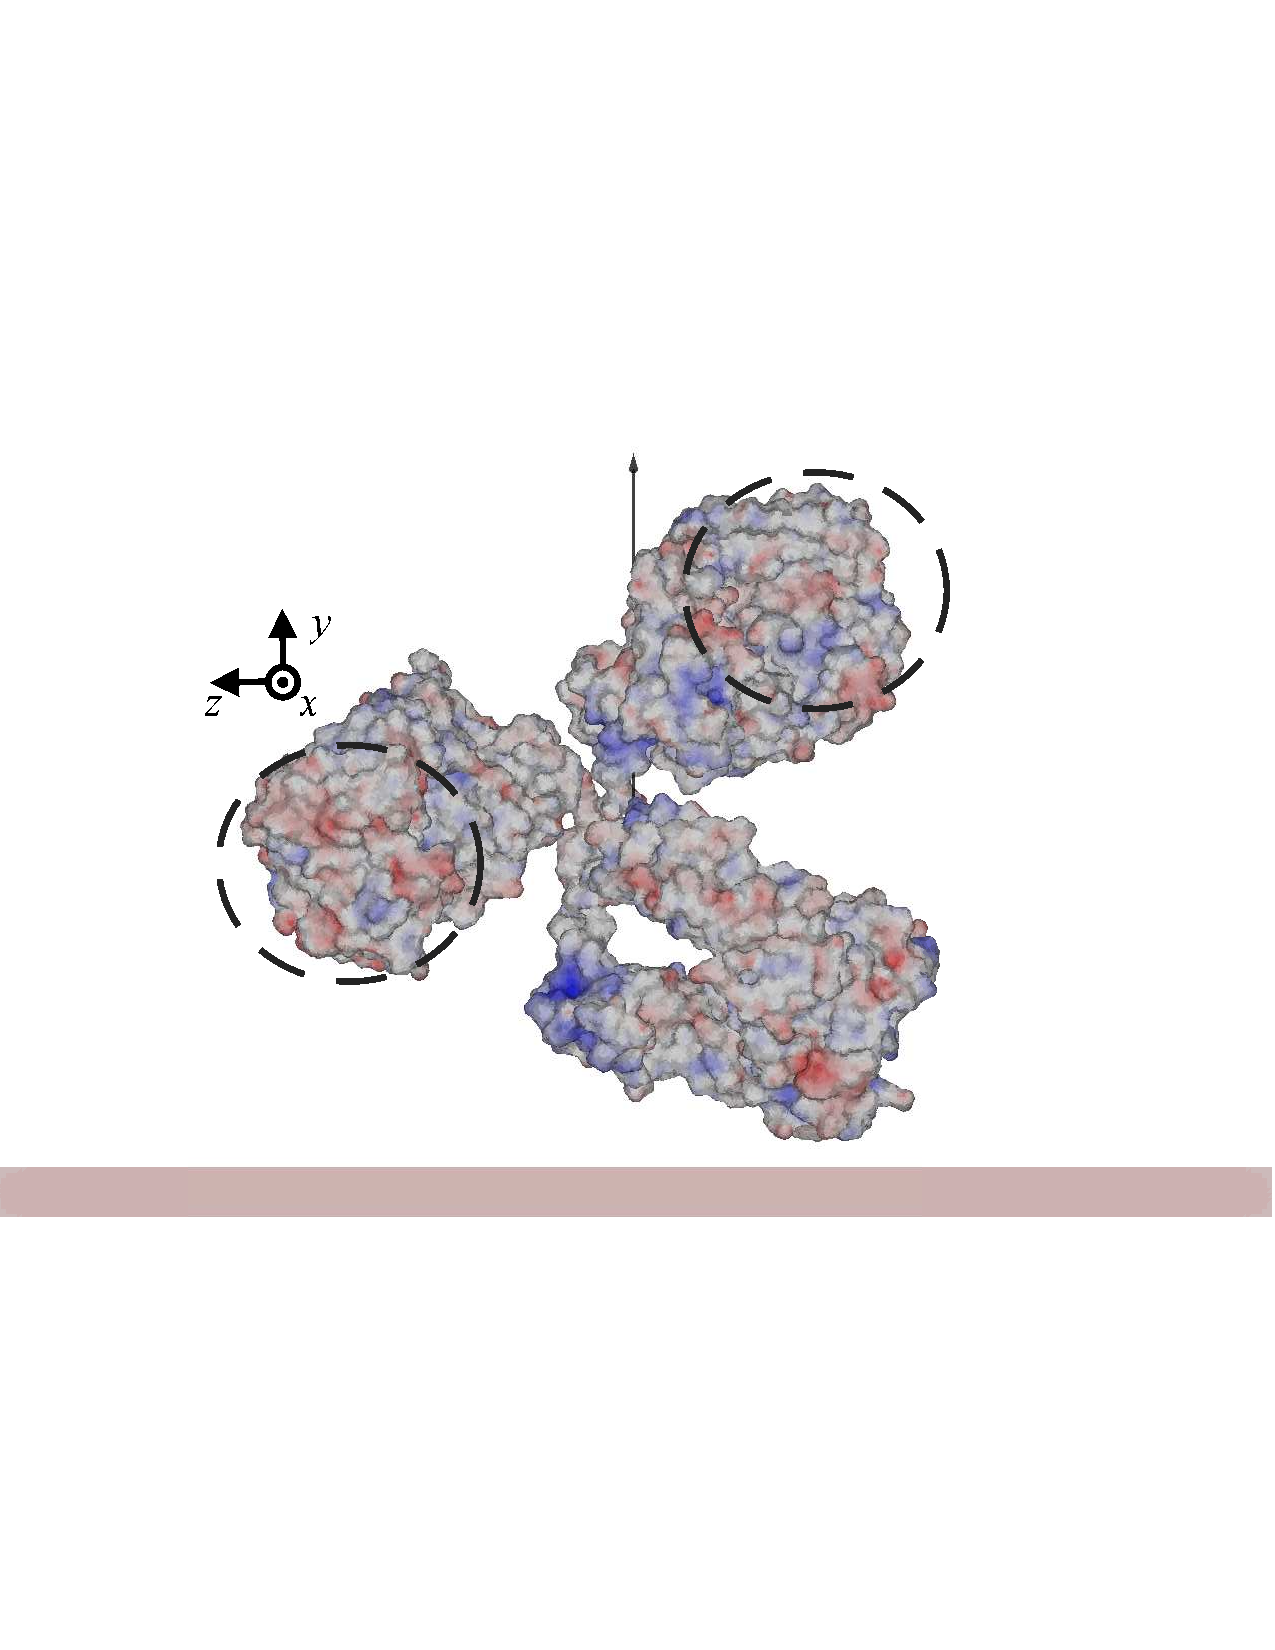
\includegraphics[width=0.4\textwidth]{Figure15f.pdf} \label{fig:1IGT_3D_sig005_kap003125_til044-rot120}}\\
   \subfloat[Probability for $\sigma$=0.2C/m$^2$ and $\kappa$=0.03125\AA$^{-1}$]{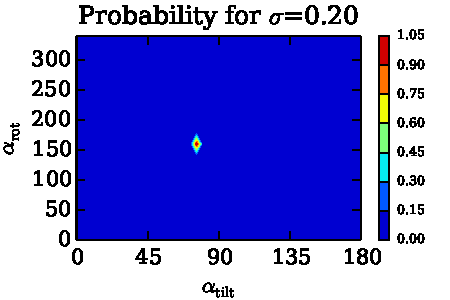
\includegraphics[width=0.4\textwidth]{Figure15g.pdf} \label{fig:1IGT_2D_sig020_kappa003125}}
   \subfloat[Side view for $\alpha_{\text{tilt}} = 76^{\circ}$ and $\alpha_{\text{rot}} = 160^{\circ}$]{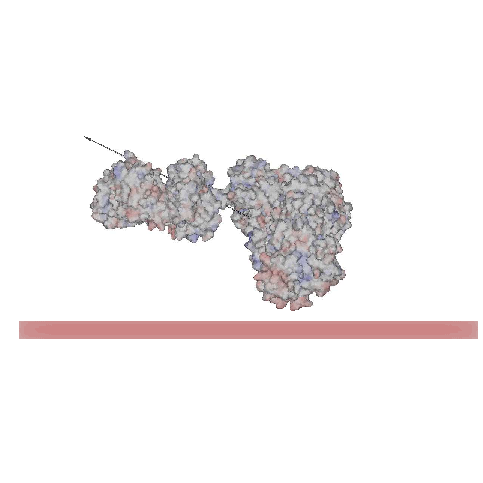
\includegraphics[width=0.4\textwidth]{Figure15h.pdf} \label{fig:1IGT_3D_sig02_kap003125_til076-rot160}}
   \caption{Orientation probability distribution and surface potential of the preferred orientation for Immunoglobulin G near a positive surface charge. The black arrow indicates the direction of the dipole moment. Data sets, figure files and plotting scripts available under \ccby.\cite{CooperBarba2015-share1348801}}
   \label{fig:1IGT_poscharge}
\end{figure*}


%%% COMMENTED OUT SECTION
\begin{comment}
\begin{figure*}
   \centering
   \subfloat[]{\includegraphics[width=0.45\textwidth]{1IGT_cos.pdf} \label{fig:1IGT_cos}}
   \subfloat[]{\includegraphics[width=0.45\textwidth]{1IGT_alpha.pdf} \label{fig:1IGT_alpha}}\\
   \subfloat[]{\includegraphics[width=0.45\textwidth]{1IGT_2D_sig005.pdf} \label{fig:1IGT_2D_sig005}}
   \subfloat[]{\includegraphics[width=0.45\textwidth]{1IGT_2D_sig-005.pdf} \label{fig:1IGT_2D_sig-005}}
   \caption{Orientation distribution of immunoglobulin G. Figures \ref{fig:1IGT_cos} and \ref{fig:1IGT_alpha} are the probability with respect to the tilt angle and its cosine, respectively. Figures \ref{fig:1IGT_2D_sig005} and \ref{fig:1IGT_2D_sig-005} are the orientation with respect to both the tilt and rotation angle.}
   \label{fig:1IGT_probability}
\end{figure*}

\begin{figure*}
   \centering
   \subfloat[Side view for $\alpha_{\text{tilt}} = 116^{\circ}$ and $\alpha_{\text{rot}} = 100^{\circ}$]{\includegraphics[width=0.45\textwidth]{1IGT_3D_sig-005_til116_rot100_side.pdf} \label{fig:1IGT_sig-005_side}}
   \subfloat[Top view for $\alpha_{\text{tilt}} = 116^{\circ}$ and $\alpha_{\text{rot}} = 100^{\circ}$]{\includegraphics[width=0.45\textwidth]{1IGT_3D_sig-005_til116_rot100_top.pdf} \label{fig:1IGT_sig-005_top}}\\
   \subfloat[Side view for $\alpha_{\text{tilt}} = 64^{\circ}$ and $\alpha_{\text{rot}} = 280^{\circ}$]{\includegraphics[width=0.45\textwidth]{1IGT_3D_sig005_til064_rot280_side.pdf} \label{fig:1IGT_sig005_side}}
   \subfloat[Top view for $\alpha_{\text{tilt}} = 64^{\circ}$ and $\alpha_{\text{rot}} = 280^{\circ}$]{\includegraphics[width=0.45\textwidth]{1IGT_3D_sig005_til064_rot280_top.pdf} \label{fig:1IGT_sig005_top}}
   \caption{Surface potential for Immunoglobulin G for the preferred orientation according to Figure  \ref{fig:1IGT_probability} for $\sigma$=-0.05 C/m$^2$ in Figures \ref{fig:1IGT_sig-005_side} and \ref{fig:1IGT_sig-005_top} and $\sigma$=0.05 C/m$^2$ in Figures \ref{fig:1IGT_sig005_side} and \ref{fig:1IGT_sig005_top}. The black arrow indicates the direction of the dipole moment.}
   \label{fig:1IGT_3D}
\end{figure*}
\end{comment}
%%% END COMMENT


%%% COMMENTED OUT SECTION
\begin{comment} 

\subsection{Fc-protein G complex} \label{sec:FCC}

We simulated the electrostatic field of the complex generated by the Fc fragment of immunoglobulin G and protein G B1 interacting with a $250\times10\times250$\AA \xspace block with surface charge density $\pm$0.05C/m$^2$, to find its preferred orientation. The protein was centered with respect to a  $250\times250$\AA \xspace face, 5\AA \xspace above it, and the orientation was defined by $\alpha_{\text{tilt}}$ and $\alpha_{\text{rot}}$, like in Section \ref{sec:PGB}. 

In these cases, we considered a 0.150M of salt in the solvent, i.e. $\kappa=0.125$, with relative permittivity 80. The region inside the protein had a relative permittivity of 4.

 \paragraph*{Mesh refinement study for Fc-protein G complex}

Similar to Section \ref{sec:PGB}, we performed a mesh refinement study to make sure the geometry was well resolved and to find appropriate simulation parameters for sampling different orientations. 

In these runs, we evaluated the solvation energy and surface energy of a system with a surface with charge density 0.05C/m$^2$, and a protein with $\alpha_{\text{tilt}} = 100^{\circ}$ and $\alpha_{\text{rot}} = 45^{\circ}$. Using the results from runs with mesh density 2, 4, and 8 elements per square Angstrom, we added the solvation and surface energies, and extrapolated them using Richardson extrapolation to obtain -1390.59 kcal/mol, with observed order of convergence 1.1. This value is the reference to calculate the errors in Figure \ref{fig:1FCC_convergence}. 

For the mesh refinement study, we used 1 Gauss points per far-away element, 19 Gauss points per close-by element, and 9 Gauss points per triangle side for the singular integral. The treecode had 6 terms in the Taylor expansion, a multipole-acceptance criterion of 0.5, and no more than 1000 boundary elements per box of the lowest level of the tree. Also, the GMRES tolerance was 10$^{-4}$. 

\begin{figure}[h] %  figure placement: here, top, bottom, or page
   \centering
   \includegraphics[width=0.5\textwidth]{1FCC_convergence.pdf} 
   \caption{Mesh convergence study of the solvation plus surface energy for the Fc-protein G complex interacting with a surface with charge density 0.05C/m$^2$.}
   \label{fig:1FCC_convergence}
\end{figure}

Figure \ref{fig:1FCC_convergence} show errors that are decaying as $1/N$ for both the solvation and surface energies, indicating that the geometry is well resolved.

 \paragraph*{Probing orientation of Fc-protein G complex}

We sampled the total free energy every $\Delta \alpha_{\text{tilt}} = 2^\circ$ of tilt angle and $\Delta \alpha_{\text{rot}} =20^\circ$ of rotation angle.  In these runs, meshes had 2 triangles per square angstrom throughout. We used 1 Gauss point per element further away than 2L of the collocation point, 19 Gauss points for close-by elements, and 9 Gauss points per side of the singular element. The treecode used 2 terms in the Taylor expansion, a multipole-acceptance criterion of 0.5 and no more than 300 elements per lowest level box. The GMRES tolerance was 10$^{-4}$. 

The total free energy was the input for numerically computing the integrals in Equation \eqref{eq:prob_angle} with the trapezoidal rule. Figure \ref{fig:probability} shows the probability of the protein orientation in terms of $\cos(\alpha_{\text{tilt}})$, in intervals of $\Delta \cos(\alpha_{\text{tilt}}) = 0.05$ for Figure \ref{fig:1FCC_cos}, and $\Delta \alpha_{\text{tilt}}$=4$^{\circ}$ for Figure \ref{fig:1IGT_alpha}.  

\begin{figure*}
   \centering
   \subfloat[]{\includegraphics[width=0.45\textwidth]{1FCC_cos.pdf} \label{fig:1FCC_cos}}
   \subfloat[]{\includegraphics[width=0.45\textwidth]{1FCC_alpha.pdf} \label{fig:1FCC_alpha}}\\
   \subfloat[]{\includegraphics[width=0.45\textwidth]{1FCC_2D_sig005.pdf} \label{fig:1FCC_2D_sig005}}
   \subfloat[]{\includegraphics[width=0.45\textwidth]{1FCC_2D_sig-005.pdf} \label{fig:1FCC_2D_sig-005}}
   \caption{Orientation distribution of Fc-protein G complex. Figures \ref{fig:1FCC_cos} and \ref{fig:1FCC_alpha} are the probability with respect to the tilt angle and its cosine, respectively. Figures \ref{fig:1FCC_2D_sig005} and \ref{fig:1FCC_2D_sig-005} are the orientation with respect to both the tilt and rotation angle.}
   \label{fig:1FCC_probability}
\end{figure*}

\begin{figure*}
   \centering
      \subfloat[Side view for $\alpha_{\text{tilt}} = 20^{\circ}$ and $\alpha_{\text{rot}} = 160^{\circ}$]{\includegraphics[width=0.49\textwidth]{1FCC_sig005.pdf}\label{fig:1FCC_sig005}} 
   \subfloat[Side view for $\alpha_{\text{tilt}} = 120^{\circ}$ and $\alpha_{\text{rot}} = 20^{\circ}$]{\includegraphics[width=0.49\textwidth]{1FCC_sig-005.pdf} \label{fig:1FCC_sig-005}}
   \caption{Surface potential for Fc-protein G complex in the preferred orientation according to Figure \ref{fig:1FCC_probability} for $\sigma$=0.05 C/m$^2$ in Figure \ref{fig:1FCC_sig005}, and $\sigma$=-0.05 C/m$^2$ in Figure \ref{fig:1FCC_sig-005}. The black arrow indicates the direction of the dipole moment.}
   \label{fig:1IGT_3D}
\end{figure*}

%%% END COMMENT OUT
\end{comment} 


\subsection{Reproducibility and data management}
To facilitate the replication of our work, we consistently release code and data associated with every publication. In that context, \pygbe was released under an MIT open-source license with our previous publication \cite{CooperBardhanBarba2013}, and continues to be available via its version-control repository. 
Supplementing this paper, we prepared \emph{``reproducibility packages''} containing running and post-processing scripts in Python to generate Figures \ref{fig:error_sphere} and \ref{fig:convergence_1PGB_sensor}. The packages invoke \pygbe with the parameters and meshes reported here, and then produce the plots, all with a single command.
The reproducibility packages are hosted on \textbf{figshare}, and are referenced in the respective captions.

\section{Discussion} \label{sec:discussion}
%!TEX root = CooperBarba-orientation.tex

\subsection{First case: protein G\,B1\,D4$^\prime$} \label{sec:disc_1PGB}

The orientation of protein \gb near charged surfaces was studied using a combined Monte Carlo and molecular dynamics method by Liu and co-workers\cite{LiuLiaoZhou2013} and experimentally by Baio and co-workers.\cite{BaioWeidnerBaughGambleStaytonCastner2012} The availability of these published results was a motivation to use this protein for a first test, to compare with the results obtained with our model. 

The results presented in Figure \ref{fig:1PGB_probability} show that for the most likely orientations, the dipole-moment vector is aligned with the vector normal to the interacting surface. This indicates that the dipole moment is the dominant effect that determines the protein's orientation, over local protein-surface  interactions. This is the expected result, since protein \gb is a relatively small biomolecule. 

Moreover, Figure \ref{fig:1PGB_probability} reveals that protein \gb behaves like a point dipole, as the most likely orientations shift 180$^\circ$ when the sign of the surface charge is flipped. This is also explained by the dipole moment dominating the orientation.
In fact, we repeated this whole set of calculations but placing protein \gb at a greater distance, 5\AA~ away from the surface, and the results did not vary.

The dipolar behavior described by our results agrees with the experiments done by Baio and co-workers, \cite{BaioWeidnerBaughGambleStaytonCastner2012} in which they observed opposite orientations of protein \gb adsorbed on NH$_3^+$ and COO$^-$ self-assembled monolayers. With positively charged surfaces, most of the proteins oriented with the N-terminal of the protein pointing away from the surface, while for negatively charged surfaces the opposite occurred, with the C-terminal pointing away from the surface. This agrees with our results in Figure \ref{fig:1PGB_probability} (the dipole moment vector of protein \gb points from the C-terminal to the N-terminal).

Liu and co-workers \cite{LiuLiaoZhou2013} used a combined Monte Carlo and molecular dynamics method to obtain $<\cos(\alpha_{\text{tilt}})>=0.95$ for $\sigma = 0.05$C/m$^2$, and $<\cos(\alpha_{\text{tilt}})>=-0.85\pm0.05$ for $\sigma = -0.05$C/m$^2$, which agrees well with our results in Table \ref{table:avg}. Note that MD simulations consider van der Waals interactions and conformational changes of the protein, whereas these are not considered in our approach, explaining the slight differences in $<\cos(\alpha_{\text{tilt}})>$.
However, as noted by other researchers,\cite{ZhouChenJiang2003,BaioWeidnerBaughGambleStaytonCastner2012,LiuLiaoZhou2013} electrostatic effects often dominate protein-surface interactions and drive orientation during adsorption, while van der Waals effects play a role only in cases of very low surface charge. For example, in Ref.~\onlinecite{ZhouChenJiang2003}, van der Waals effects were of consequence in a setup with surface charge of 0.006C/m$^{2}$ and high ionic strength, leading to weak electrostatics. In a biosensor-fabrication scenario, this would only be the case with low-quality \sam s.

The results with protein \gb mean that an electrostatic solver with implicit solvent using the Poisson-Boltzmann equation is capable of capturing the driving mechanism of physical adsorption and orientation of the adsorbed molecule, at least in cases where the molecule's dipole moment is dominating the orientation. This is important because protein adsorption, being a free energy-driven process, is difficult to study experimentally\cite{MijajlovicETal2013} and thus simulations offer a promising alternative. Full atomistic molecular dynamics, however, demands large amounts of computing effort, and the possibility of using an electrostatics solver may extend the range of systems that can be investigated.


 \subsection{Second case: immunoglobulin G}

With our numerical model already verified using an analytical solution for spherical geometry\cite{CooperBarba2015a} and the successful results for protein orientation of a small protein near a charged surface (Section \ref{sec:disc_1PGB}), we proceeded to study the effect of surface charge and salt concentration on the orientation of the antibody immunoglobulin G. Antibodies are widely used in biosensors as ligand molecules, due to their affinity and specificity with the target molecule (antigen), and it is vitally important that they are adsorbed on the sensor with the antigen-binding Ig fragment (Fab) pointing away from the sensor, into the oncoming flow containing the antigens (known as ``end-on'' or ``tail-on'' orientation).
Early experimental studies found that antigen/antibody ratio was especially low on negatively charged surfaces,\cite{BuijsETal1997} leading to the notion that protein orientation was affected to leading order by charge. 
One subsequent study\cite{ChenLiuZhouJiang2003} investigated the orientations of two iso-types of immunoglobulin G---\ig 1, corresponding to \pdb\ structure {\small 1IGY}, and \ig 2a, corresponding to \pdb\ {\small 1IGT}---adsorbed on positive and negatively charged surfaces. 
As an indirect method of probing antibody orientation, the researchers obtained adsorbed amounts and antigen/antibody ratios by means of surface-plasmon resonance experiments (e.g., a higher antigen/antibody ratio would indicate that more active sites are accessible and more antibodies are in a favorable orientation). 
The finding was that \ig 1 mainly had a ``head-on'' (unfavorable) orientation on the negatively charged surfaces and a mix of ``tail-on'' (most favorable) and ``side-on'' orientations on the positively charged surfaces. 
\ig 2a, on the other hand, had many orientations on both surfaces with positive and negative charge, leading to the conclusion that \ig 2a is harder to control using electrostatic effects.
Results consistent with these were obtained by Zhou and co-workers\cite{ZhouChenJiang2003} using a united-residue model: a coarse-grained model where each amino-acid is treated as a sphere. They find that \ig 1 will have the favorable ``end-on'' orientation on positive surfaces, as long as the charge density was large enough (0.018C/m$^{2}$, in their case) and the ionic strength was low. But \ig 2a  did not show a clear preferred orientation at the conditions they looked at; the authors attribute this to the weaker dipole moment of this iso-type.
 
We investigated the orientation of \ig 2a, which other studies found harder to orient favorably on a biosensor surface, and used two values of the surface charge ($\sigma=0.05$ and $0.1$C/m$^{2}$) and two values of salt concentration ($\kappa=0.125$ and $0.0625$\AA$^{-1}$), in each case varying two-fold.
 Figures \ref{fig:1IGT_negcharge} and \ref{fig:1IGT_poscharge} present the probability distribution of \ig 2a for many orientations (given by $\alpha_\text{tilt}$ and $\alpha_\text{rot}$), in each case.
 The following discussion refers to each variation of the parameters and the effect on the preferred orientation of the adsorbed antibody and its probability.

 \medskip
 
 \paragraph*{Effect of surface charge---}
 
The lower value of surface charge here is $\sigma=\pm 0.05$C/m$^2$, the same value used in Ref.~\onlinecite{LiuLiaoZhou2013} to mimic the experiments reported in Ref.~\onlinecite{BaioWeidnerBaughGambleStaytonCastner2012}. 
Figures \ref{fig:1IGT_2D_sig-005} and \ref{fig:1IGT_2D_sig005} show that for the lower value of surface charge with the higher salt concentration ($\kappa=0.125$\AA$^{-1}$), there is no clear preferred orientation, to the point that the highest probability falls under 10\%. 
This means that adsorbing the antibodies under these conditions would result in a wide range of orientations, which would not be favorable for biosensor fabrication.
Moreover, the preferred configurations in figures \ref{fig:1IGT_2D_sig-005} and \ref{fig:1IGT_2D_sig005} show the antibody lying flat on the surface, far from the desired ``tail on'' orientation. 
This observation is consistent with a previous study using a unified-residue model,\cite{ZhouChenJiang2003} where this particular antibody showed many possible orientations. 
The authors of that study attributed this behavior to the weaker dipole moment of this molecule, compared with the variant \ig 1.
 
With the higher value of surface charge, in this case $\sigma=\pm0.1$C/m$^2$, the orientation probability distribution in the case of negative charge improves somewhat, as the antibody is slanted sideways rather than lying down (at least one antingen-binding fragment is pointing up), and the probability of the preferred orientation is almost doubled for low salt concentration.
For positive surface charge the slanted orientation is similar, however the probability is higher for the preferred orientation in both the low- and high-salt cases.
In the cases with higher salt concentration, Figure \ref{fig:1IGT_2D_sig020_kappa01250} shows a preferred orientation with a higher probability of 12\%, compared to 8\% in Figure \ref{fig:1IGT_2D_sig005}, and the dipole moment rotates towards the normal vector. 
For the lower value of salt concentration (Figure \ref{fig:1IGT_2D_sig020_kappa003125}), this effect is smaller, however it shifts the preferred tilt angle in the opposite direction, from $44^{\circ}$ to $64^{\circ}$. Note that the dipole-moment vector does not point straight through the middle between the two Fab fragments, but in an angle.
This indicates that, in contrast to protein \gb, local interactions dominate over the dipole moment. If the dipole moment were the dominant effect, the dipole-moment vector would tend to align to the surface normal as the surface charge increases.
This argues against the suggestion by other researchers\cite{ChenLiuZhouJiang2003,ZhouChenJiang2003} that the dipole-moment vector is the main determinant of orientation.
 
 \medskip
 
 \paragraph*{Effect of salt concentration---}
 
As the surface charge density was varied two-fold, we also varied the Debye length ($\kappa^{-1}$) two-fold. In terms of salt concentration, it means a 4$\times$ decrease in the amount of salt. The higher value of salt concentration corresponds to 145mM, which is in the physiological salt range.  
 
Like increasing the surface charge, lowering the salt concentration affects the orientation probability distribution. 
 For $\sigma=-0.05$C/m$^2$ (Fig.~\ref{fig:1IGT_2D_sig-005_kappa003125}), the effect is a large shift in the preferred tilt angle, from $\alpha_\text{tilt}=116^\circ$ to $\alpha_\text{tilt}=40^\circ$, with a small change in probability. 
For the positive weaker charge, $\sigma=0.05$C/m$^2$ (Fig.~\ref{fig:1IGT_2D_sig005_kappa003125}), not only does the peak probability increase considerably ($\sim 3\times$), but the preferred tilt shifts from $64^{\circ}$ to $44^{\circ}$.
This orientation is favorable for biosensing applications, as the antigen-binding fragments are pointing away from the surface, in a ``tail on'' orientation.
 For the stronger negative charge, $\sigma=-0.1$C/m$^2$, the probability peak increases  $2.5\times$ for a slanted orientation where one of the antigen-binding fragments is attached to the surface in an unfavorable position (Fig.~\ref{fig:1IGT_2D_sig-020_kappa003125}).
 With positive surface charge, the tilt angle shifts in such a way that the antibody is lying on the surface with a marked probability close to $30\%$ (Fig.~\ref{fig:1IGT_2D_sig020_kappa003125}).
 This orientation is not ideal for biosensors, but it is better than the slanted position as neither of the Fabs are attached to the surface.

From the results in Figures \ref{fig:1IGT_negcharge} and \ref{fig:1IGT_poscharge}, we see that the iso-type \ig 2a can be better controlled in orientation with low salt concentration and high surface charge, as we get more pronounced high-probability regions. 
Moreover, good orientations for biosensors are more likely to occur with positive surface charge (Figure Figures \ref{fig:1IGT_3D_sig-02_kap003125_til124-rot140}), since the Fab fragments are pointing up.
Previous studies had shown that the \ig 1 variant could be controlled, but not \ig 2a. 
The advantage of a positive surface charge and a low ionic strength had been suggested by previous studies, but not for this particular variant of immunoglobulin G. Note also that our lower value of salt concentration is 37mM, which is a higher amount of salt than other studies.\cite{BuijsETal1997,ChenLiuZhouJiang2003}


The main limitation of this study stems from the application of linearized Poisson-Boltzmann equation.
Bu and co-workers\cite{BuVakninTravesset2006} assessed the accuracy of the Poisson-Boltzmann equation for highly charged surfaces ($\sim 0.4$C/m$^2$), getting good agreement of the model with experiments. 
Rigurously, the linearized Poisson-Boltzmann equation is a valid approximation of the Poisson-Boltzmann equation when the nondimensional potential is smaller than 1 ($\phi q_e/k_BT<<1$), however, in molecular simulations this restriction can be somewhat relaxed for solvation energy calculations. 
For example, we ran a calculation on an isolated \ig 2a immersed in a solvent with 37mM of salt ($\kappa = 0.0625$), using our boundary element code with the parameters from Table \ref{table:params5}. 
In that calculation, we obtained that the absolute value of the dimensionless potential on the molecular surface averaged 1.5, and over $55\%$ of the triangles had $\phi q_e/k_BT>1$.
Then, we compared the solvation energy of the isolated \ig 2a obtained with the linear and non-linear Poisson-Boltzmann models using APBS.\cite{BakerETal2001} In this case, the volumetric mesh spanned $150\times 150\times 150$\AA\ with 449$^3$ nodes, and the energies differed by $0.02\%$.
This observation is consistent with the results from Ref.~\onlinecite{Fogolari99}, where they get good agreement between linear and non-linear Poisson Boltzmann when the average dimensionless potential on the molecular surface is between -2 and 2. The same authors also compared the two models for solvation energy calculations of nucleic acids, which are highly charged.\cite{FogolariETal2015} In that work, they made a distinction between the salt-dependent and salt-independent contributions to solvation energy, concluding that linear Poisson-Boltzmann accurately reproduced the salt-dependent contributions to solvation energy only for concentrations above 0.1M, however the total solvation energy agreed for a wide range of salt concentrations. 
Placing a surface with charge $\sigma=0.1$C/m$^2$ next to \ig 2a in the configuration from Fig. \ref{fig:1IGT_3D_sig02_kap003125_til076-rot160}, the average absolute value of the dimensionless potential is 1.3, and it exceeds 1 in $51\%$ of the triangles, so we can expect the linearized Poisson Boltzmann to give a good approximation of the solvation energy.

Our results suggest that a high surface charge and low salt concentration increases the probability of the preferred configuration, and that better orientations are obtained with positive surface charge.
We studied the orientation of \ig 2a near a surface with $\sigma =0.2$C/m${^2}$ and $\kappa=0.03125$\AA$^{-1}$ using our boundary element code, to see if this trend continues (Figure \ref{fig:1IGT_sigma02}). 
Even though the electrostatic potential is outside the linear regime in this case, and our model is based on the linearized Poisson-Boltzmann equation, these results show that as we increase the electrostatic effects, the preferred orientation becomes highly marked, and tends towards a favorable orientation for biosensors.

\begin{figure*}
   \centering
   \subfloat[Probability distribution]{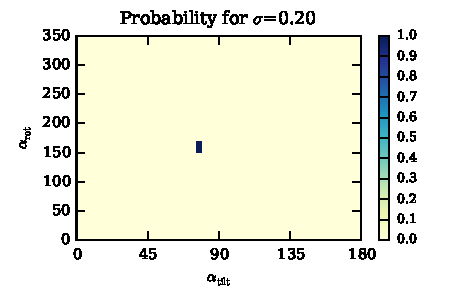
\includegraphics[width=0.4\textwidth]{Figure17a.pdf} \label{fig:1IGT_sig02}}
   \subfloat[x-y plane view for $\alpha_{\text{tilt}} = 76^{\circ}$ and $\alpha_{\text{rot}} = 160^{\circ}$]{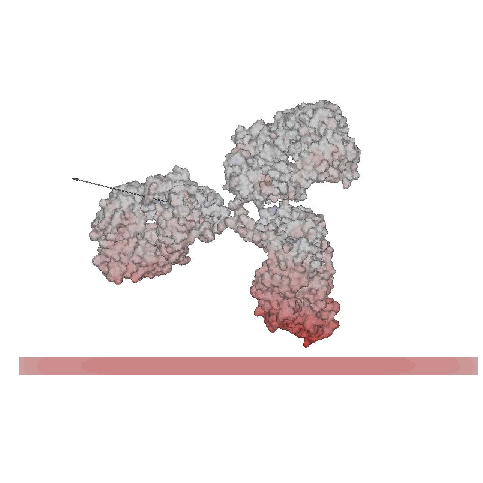
\includegraphics[width=0.4\textwidth]{Figure17b.pdf} \label{fig:1IGT_3D_sig02}}
   \caption{Orientation probability distribution and surface potential of the preferred orientation for immunoglobulin G near a surface with $\sigma=0.2$C/m$^2$ and $\kappa=0.03125$\AA$^{-1}$. Data sets, figure files and plotting scripts available under \ccby.\cite{CooperBarba2015-share1348801}}
   \label{fig:1IGT_sigma02}
\end{figure*}

\section{Conclusion}
%!TEX root = CooperBarba2014.tex

In this work, we used an implicit-solvent model to study protein-surface interaction. We present for the first time and apply an extension of our open-source \pygbe code to account for the presence of surfaces with imposed potential or charge. The new feature of the code was verified against an analytical solution, which we derived for that purpose. 

To demonstrate the power of this approach in a more realistic setting, we performed tests of protein G B1 D4$^\prime$ near a brick-shaped surface with an imposed charge. The error in energy scaling with the area of boundary elements demonstrates that this extension of \pygbe is capable of resolving the mathematical model correctly. This test was motivated by the biosensing application, where a ligand molecule is adsorbed on a \sam-coated nanoparticle, which can be represented by the brick-shaped surface.

The addition of a surface with imposed charge or potential in the implicit-solvent model falls naturally in a boundary integral approach. In this case, the region enclosed by the surface is not part of the domain, then, this surface only adds one equation to the linear system, rather than two, which is the case with the molecular solvent-excluded surface.

We conclude that this implicit-solvent model can offer a valuable approach in protein-surface interaction studies. This tool can be useful for orientation studies of ligand molecules in biosensors, either to find optimal adsorption conditions of salt concentration and surface charge, or to guide the design of better ligand molecules. 





\section*{Acknowledgments}
 This work was supported by ONR via grant \#N00014-11-1-0356 of the Applied Computational Analysis Program. LAB also acknowledges support from NSF CAREER award OCI-1149784 and from NVIDIA, Inc.\ via the CUDA Fellows Program. 
 We are grateful for many helpful conversations with members of the Materials and Sensors Branch of the Naval Research Laboratory, especially Dr. Jeff M. Byers and Dr. Marc Raphael.

% Create the reference section using BibTeX:
\bibliographystyle{elsarticle-num}
\bibliography{CompBio,bem,scicomp,fastmethods,scbib,biosensors}

\end{document}
